\documentclass[11pt]{article}
\usepackage[utf8]{inputenc}
\usepackage[margin=1in]{geometry}
\usepackage{natbib}
\usepackage{graphicx}
\usepackage{mdframed}

\title{An agent-based model for city networks based on interactions between firms}

\date{}

\begin{document}

\author{J. Raimbault$^{1,2,3}$, N. Zdanowska$^{1,3}$ and E. Arcaute$^1$\\\medskip\small
$^{1}$ Centre for Advanced Spatial Analysis, UCL; $^{2}$ UPS CNRS 3611 ISC-PIF; $^{3}$ UMR CNRS 8504 G{\'e}ographie-cit{\'e}s
}

\maketitle
% NetSci format: A4, 11pt, 1in margin, max 12p + up to 3p references

\begin{abstract}
    This paper introduces a generative model for urban networks defined by interactions between firms. The aim is to test several geographical properties emerging in such a network as metropolisation, internationalisation or regionalisation. The growth of the network is simulated by adding randomly new links defined by ownership between firms, with probabilities of occurring depending on the economic size of urban areas at origin and destination, industrial sector proximity between firms, the strength of links from the past as well as the geographical and socio-cultural distance. The simulation on a synthetic system of cities unveil phase transitions when changing interaction distance, and non-trivial patterns in the model behavior. Calibration of the model on real data on company ownership linkages for Europe in 2018 is also undertaken. Future work will consist in observing thanks to this model the impact of economic crisis on such networks.
    
    
\end{abstract}

\section{Introduction}

The intensification of globalisation of the economy since the late 20th century resulted in the rise of the network society \citep{castells2000networksociety} and the emergence of a world-city system \citep{taylor2001specification}, characterized by highly interconnected urban centres at the global level \citep{sassen1991}. These interactions can be of different nature and determined by economic, socio-cultural, or geopolitical proximity implying spatial and non spatial patterns \citep{martinus2018global}. Interactions of economic nature between transnational firms, are together with trade among the most representative of the current economic trends \citep{taylor2001specification}. Understanding the drivers of growth and geographical properties of such a urban network, can be used to foster innovation in specific cities and to shape public policies for local industrial clusters \citep{turkina2016structure}. Straightening these city-interactions can be crucial for revitalising certain regions \cite{Clarke2018}, by developing strategic industries for global insertion of regions \cite{dawley2019creating}, cities \cite{gluckler2016relational} and countries \cite{martinus2019brokerage}. The functioning of such a city-network and the position of cities within these networks \cite{gluckler2016relational} can also permit to infer the consequences of future exogenous shocks such as an economic crisis, a single market collapse or a post-Brexit scenario for the European Union.

The use of network models to understand processes underlying the emergence and dynamics of such urban networks has already been widely tackled in the literature. \cite{dai2016simulating} propose a generative urban network model at the regional scale, combining geographical factors with network topological properties. Air transportation networks can also be understood as urban networks, and \cite{zanin2013modelling} reviews several models for such networks. Trade network have been extensively studied from the viewpoint of complex networks, but are generally driven at the country-level \cite{garlaschelli2005structure} because of scarce data at city-level. Input-output models, mostly used in Regional science to represent flows between geographical areas, are considered in some cases as a type of urban generative model \cite{jin1993generation}. In this stream of research, spatial interaction models \cite{dennett2013multilevel} can form the basis of urban network models for abstract flows \cite{dai2016generative} or physical infrastructure \cite{raimbault2020indirect}.


%\citep{martinus2018global} combination of different types of proximity in inter-urban firm networks: economic, sociocultural, geopolitical - implies spatial and non-spatial 
%\citep{pan2017mapping} different types of linkages: e.g. services here, but not only. All sectors should be taken into account first.
%\cite{martinus2019brokerage} role of small countries
%\cite{dawley2019creating} regional policies for insertion in global network
%\cite{gluckler2016relational} positioning within networks


The originality of the present paper is to approach these issues within the system of cities framework \citep{berry1964cities}, where the position and dynamics of cities in the socio-economic world-wide space can be considered by their interactions with other cities \cite{pumain2018evolutionary}. We examine the interactions of European cities within firm linkages defined by corporate ownership links. Since transnational firms structure is one of the determinant of the global economic space, it provides one accurate proxy to unveil geographical structures \cite{2019arXiv191014652Z}. More precisely, our contribution relies on the following points: (i) we propose an empirical analysis of the firm ownership urban network for the European Union, based on the Bureau Van Dijk's \emph {AMADEUS} database; (ii) we introduce a generative network model to simulate the growth of such linkages at urban areas scale, which combines multiple factors influencing link formation, as economic intensity of origin and destination of urban areas, industrial sector proximity, the strength of previous links, and geographical and socio-cultural distance; (iii) the model allows us to compare the effect of different factors on the final network structure, which is extensively studied through model sensitivity analysis and exploration; and (iv) we calibrate the model on the empirical network.


The rest of this paper is organized as follows: we first proceed to an empirical analysis of the network studied. We then describe the generative model for urban networks, and its sensitivity analysis and exploration on synthetic data. We then parametrize and calibrate the model on real European firm ownership data. We finally discuss implications of our results and possible extensions.


\section{Empirical network analysis}

% stats to describe the structure of the database, nb of total links, nodes, missing values? + nb of firms per country,  total turnover generated per country etc..

Companies from the AMADEUS database are georeferenced using the Geonames database (using postcode or address depending on the information available). We then join this data with the GHS-FUA dataset for functional urban areas \cite{Florczyk2019ghs}, which are the relevant objects for applying our model. Starting from a firm-level dataset of 1,562,862 nodes and  1,866,936 links, we obtain a directed network of 573 urban areas and 9323 ownership links. Weight of links are obtained by computing the owned share of turnover at destination, i.e. $w_{ij} = \sum_{k \in i,l \in j} s_{kl} \cdot T_l$ where $s_{kl}$ of the ownership share of company $l$ by company $k$ and $T_l$ the turnover of company $l$. Node attributes include an economic size of urban areas, that we compute as the sum of turnovers of companies within the area. This quantity is highly correlated with area-level GDP included in the GHS database (Spearman correlation $\rho = 0.71$) and also with population ($\rho = 0.60$), so we expect to capture size effects while keeping the consistence of a single main data source. An other attribute of nodes is the industrial sector composition, expressed as a proportion of turnover in the area associated to a given industrial sector. Detailed sectors of firms are available up to the fourth digit for the NACE classification in the raw data. We consider the first level classification (21 categories) and compute sector proportions accordingly.

The urban network has heavy tail weighted degree and edge weight distributions, as shown in Fig.~\ref{fig:nwdist}. We fit power law and log-normal distributions, including minimal value cutoff following \cite{clauset2009power}, using the \texttt{powerlaw} R package \cite{powerlawpackage}. For both, log-normal distributions appear to be a better fit ($\mu=18.8$, $\sigma=2.3$ for weighted degree; $\mu=13.8$, $\sigma=2.8$ for edge weight), and include a much broader range of the empirical distributions with lower estimated cut-offs. These heavy tail properties suggest the relevance of a generative model including self-reinforcing processes which are known to produce such distributions.

%%%%%%%%%%%%%
\begin{figure}
    \centering
    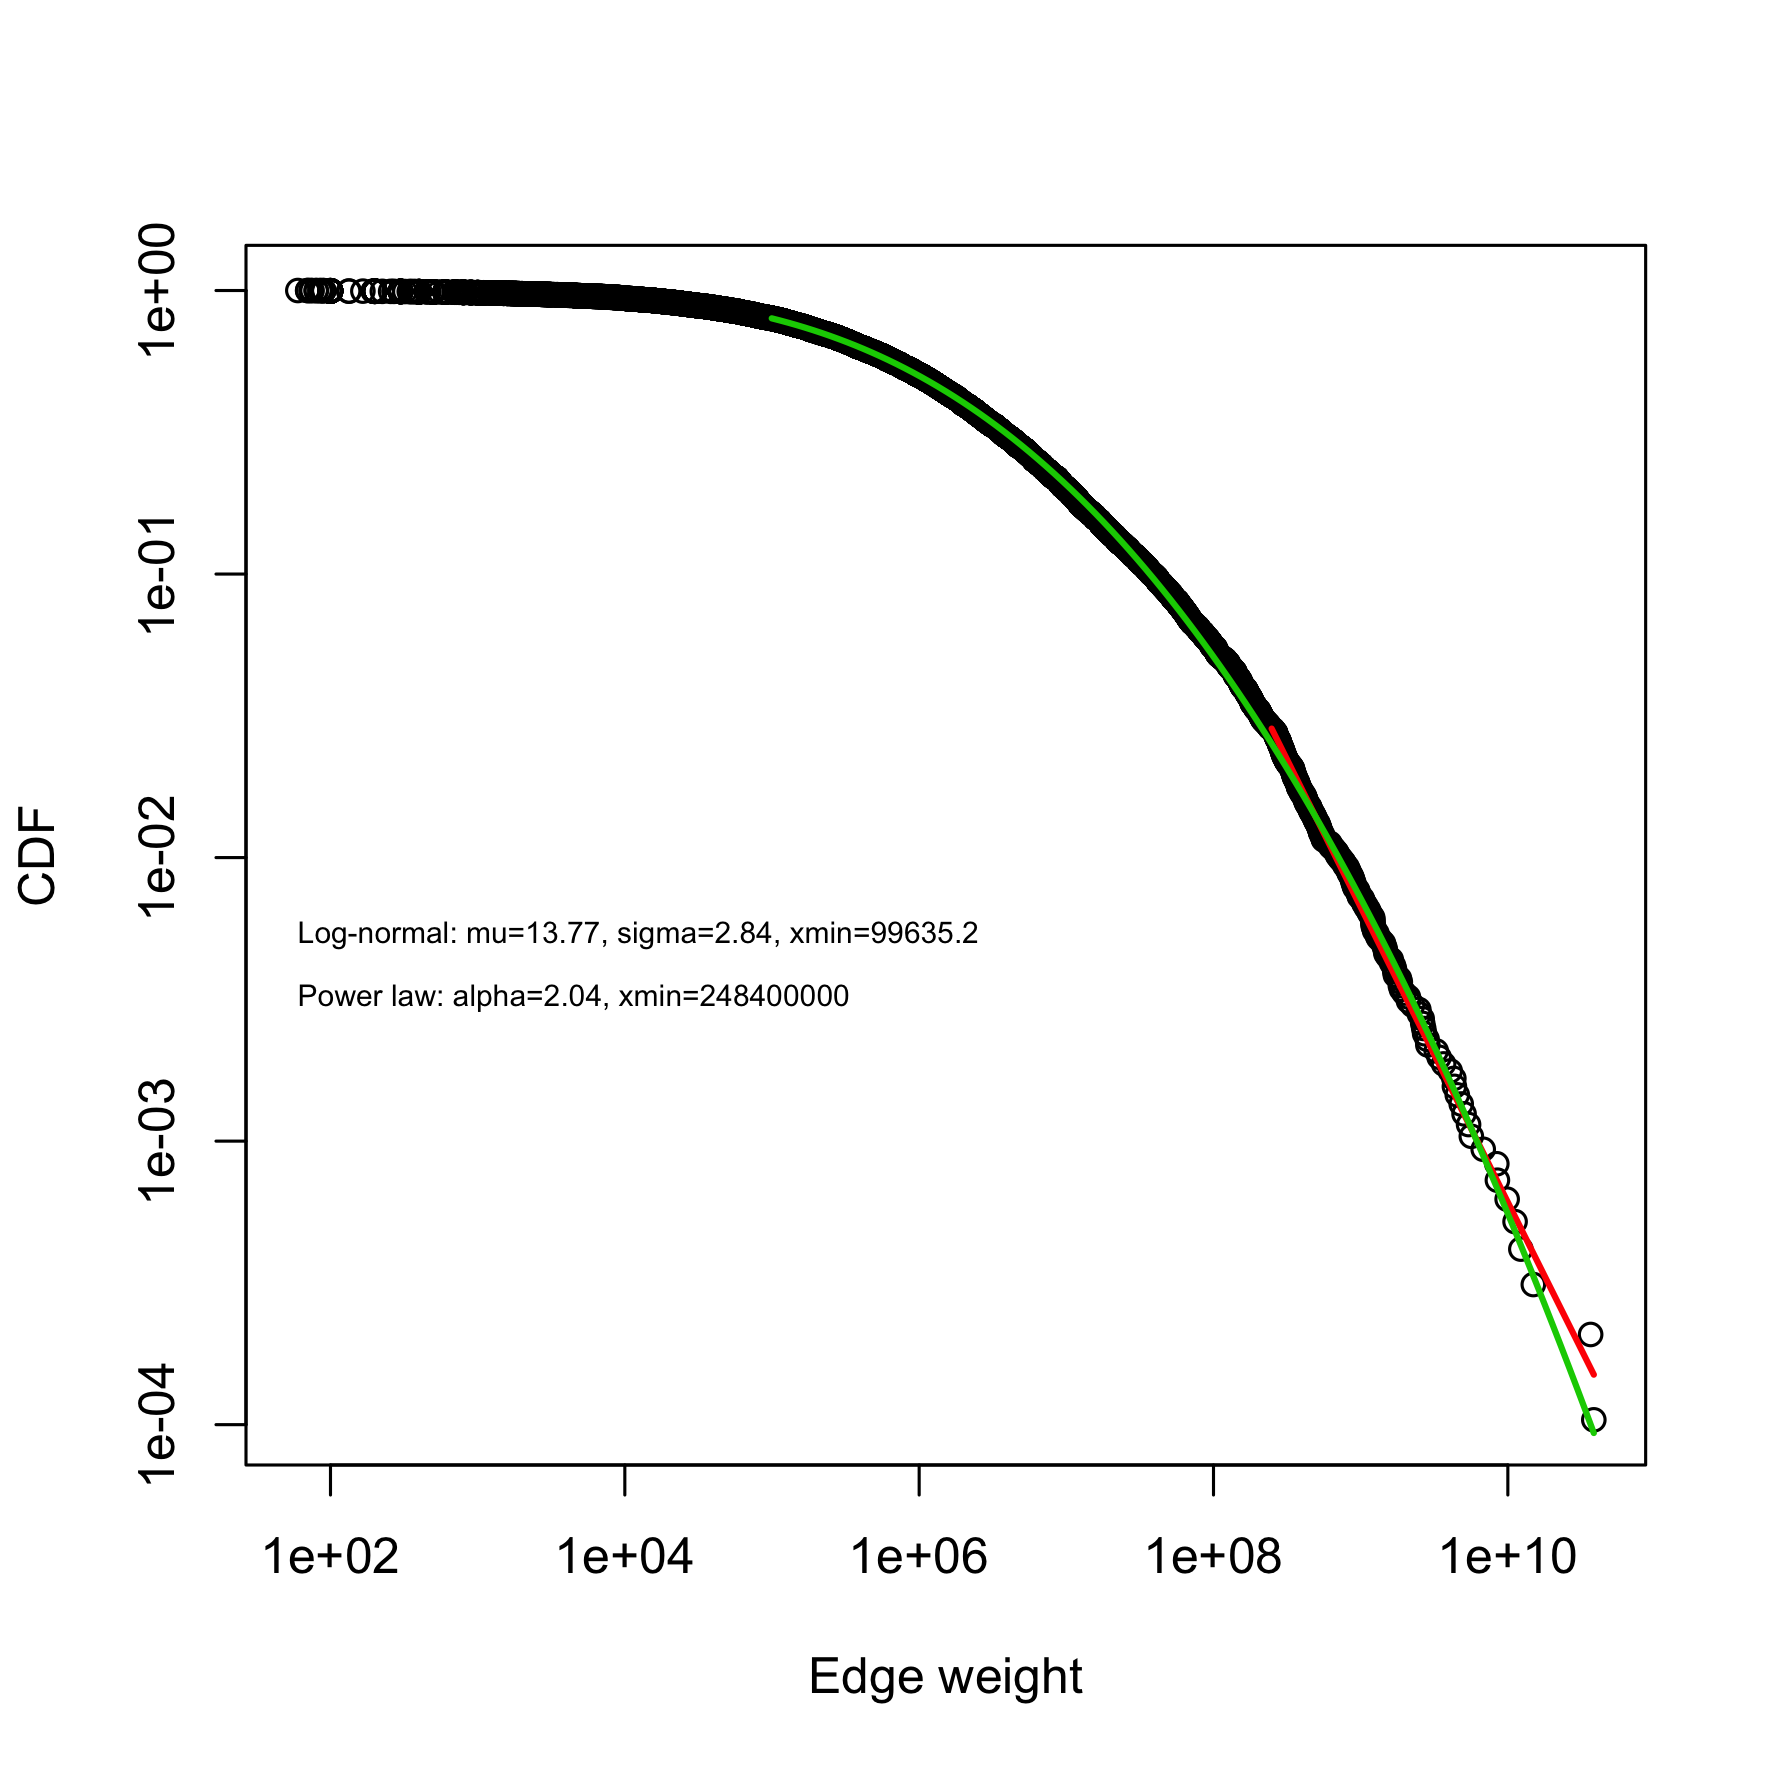
\includegraphics[width=0.49\textwidth]{figures/edgeweight.png}
    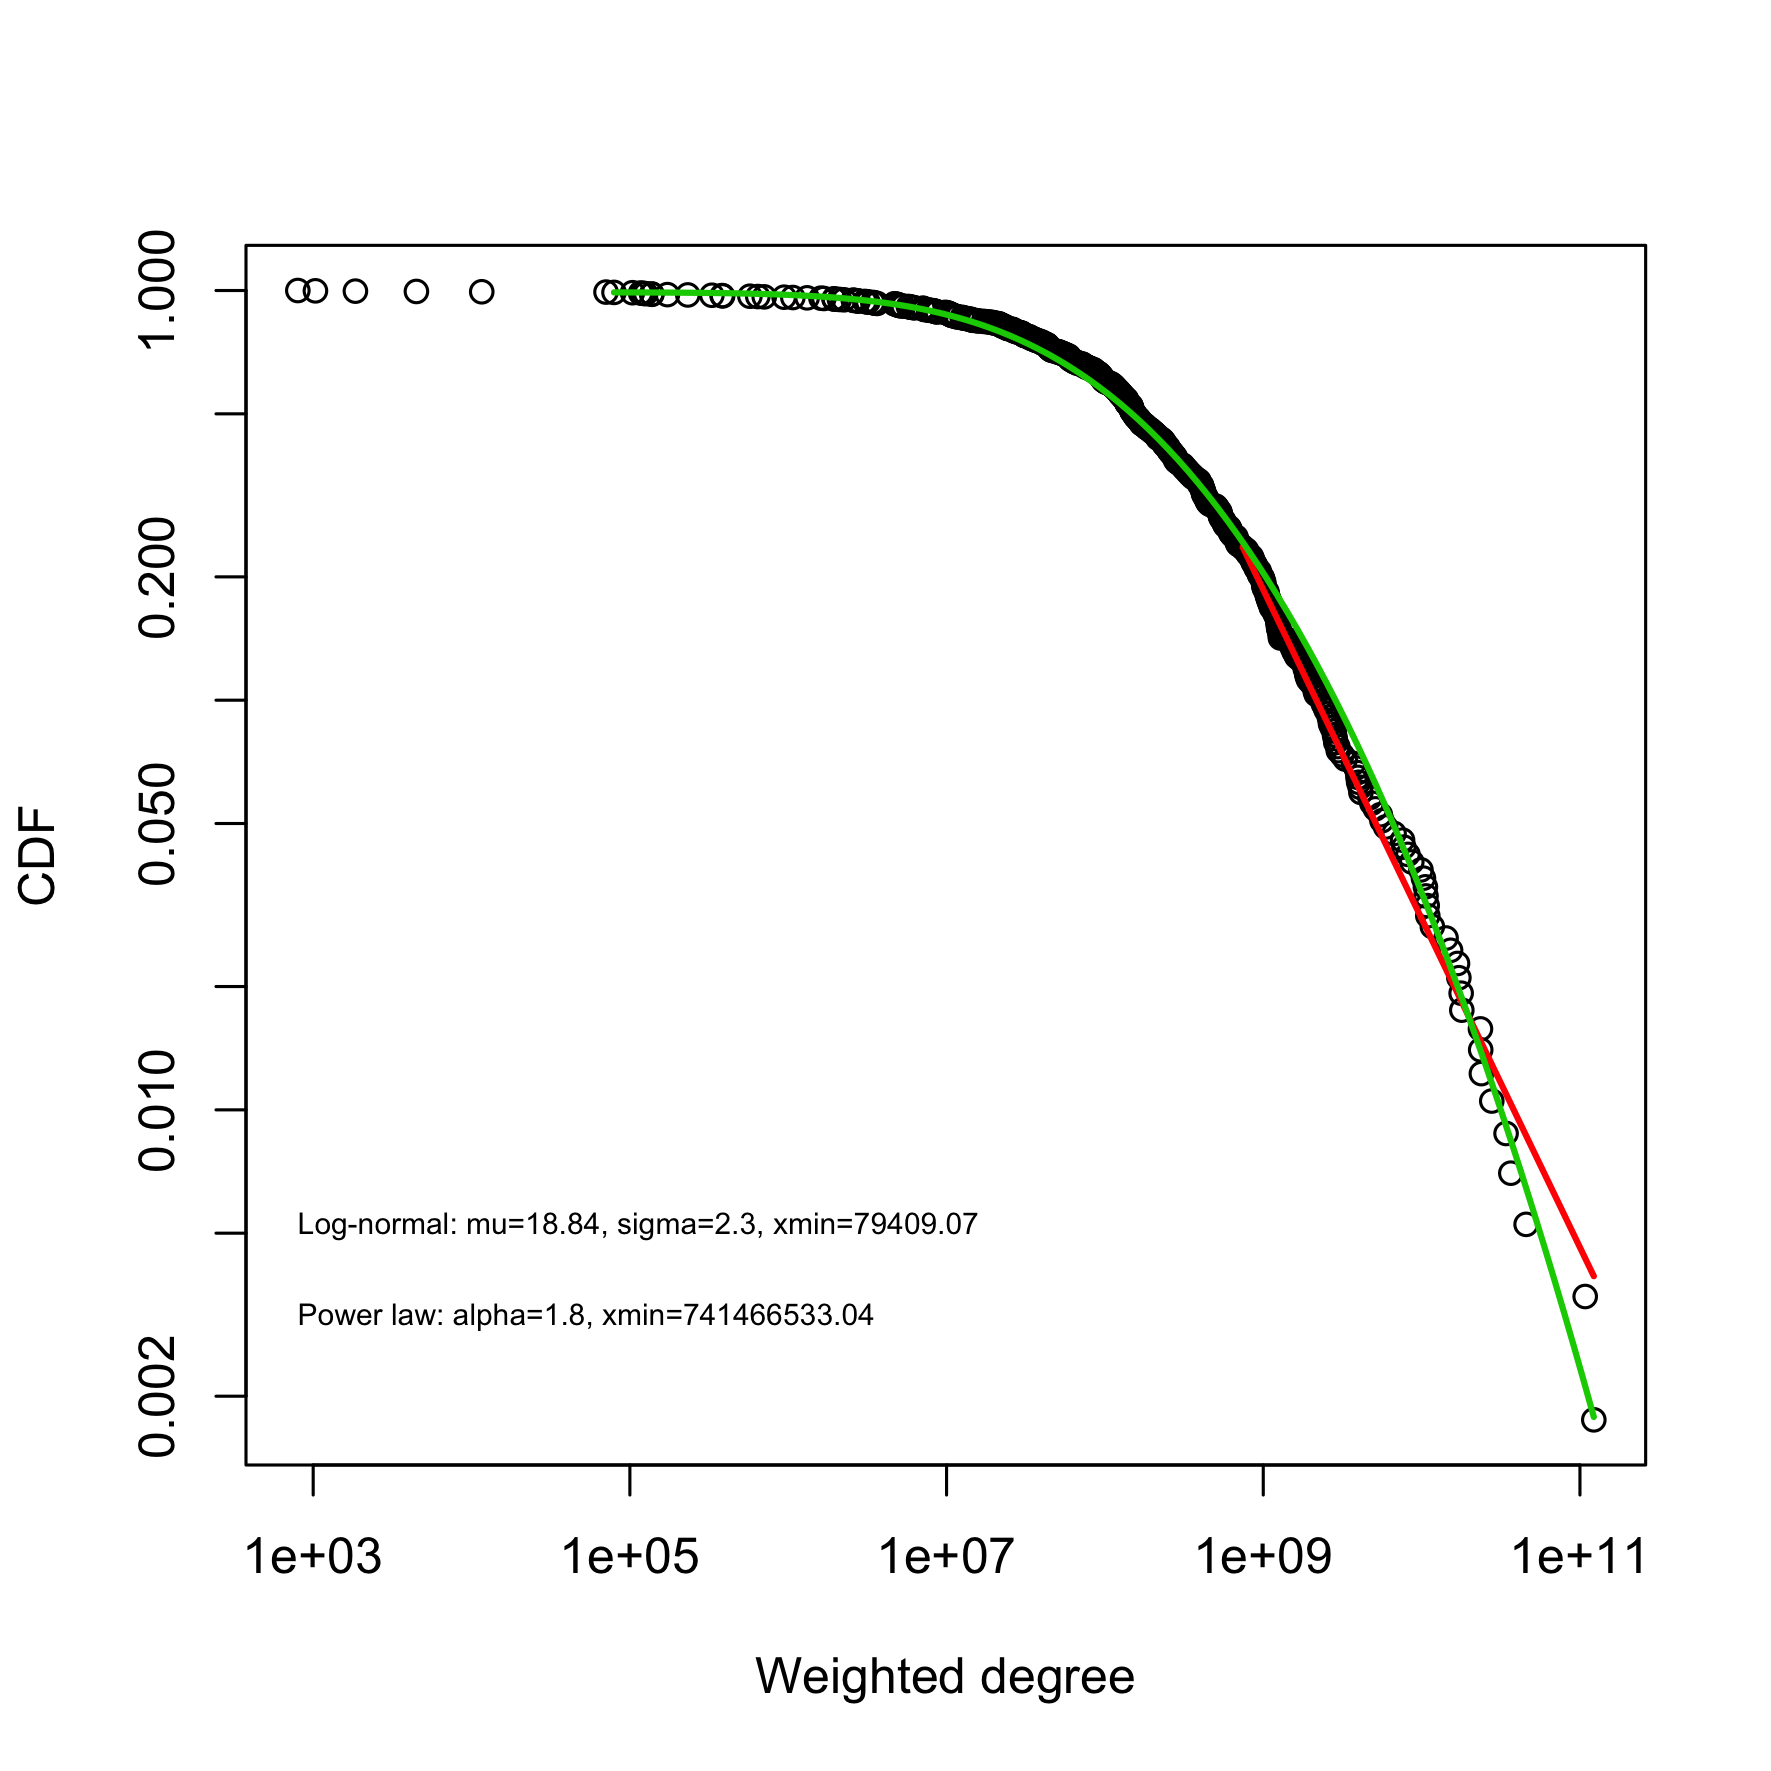
\includegraphics[width=0.49\textwidth]{figures/degreeDistr.png}
    \caption{Distributions of network properties. \textit{(Left)} Cumulated distribution for edge weight, with power law fit (red) and log-normal fit (green); \textit{(Right)} Cumulated distribution for weighted degree.}
    \label{fig:nwdist}
\end{figure}
%%%%%%%%%%%%%


Regarding the community structure of the network, different modularity maximization algorithms (run on the undirected corresponding network) give a same undirected modularity of 0.38, and a directed modularity \citep{nicosia2009extending} of 0.34 for the greedy algorithm of \citep{clauset2004finding} and 0.36 for the Louvain algorithm \citep{blondel2008fast}, corresponding to 36 communities (resp. 15). In comparison, with 29 countries, the classification of urban areas by country has a modularity of 0.32. This means that the structure of flows has a certain regional integration. Indeed, a null model assigning random labels with 30 communities, bootstrap 1000 times, yields an average modularity of $0.049 \pm 0.002$, confirming the statistical significance of these communities.


To have a first insight into factors playing a role in the formation of links, we proceed to a statistical analysis which is similar to unconstrained spatial interaction models \cite{wilson1975some}.
% poisson \cite{flowerdew1988fitting}



\section{Model}

\subsection{Rationale}

The model is expected to capture a single macroscopic urban scale, i.e. the level of the urban system where basic entities are cities. Links are induced by underlying firms but these are not explicit. Cities are defined by an economic size, but also by an industrial sector profile. As \citep{martinus2018global} point out, a combination of several distances may play a role in establishing linkages. Geographical distance and industrial proximity and complementarity will typically be in concurrence \cite{cottineau2020nested}. Therefore, we combine several processes driving network growth: (i) geographical proximity (in our case the crow-fly distance, but it can be generalized to any type of accessibility); (ii) geopolitical proximity, which captures the higher propensity to establish links within existing submarkets despite the European common market (confirmed relevant by the fixed effect regression described above); (iii) city economic size, which has furthermore scaling laws properties; (iv) industrial proximity in terms of firm sector composition; (v) previous linkages (influence of history). This last point is crucial to capture accumulated effects and include path-dependency, which fits well the use of a simulation model instead of a more simple statistical model.



\subsection{Model description}

Let $1 \leq i \leq N$ cities defined at time $t$ by their economic structure such that $E_i(t)$ is the total economic volume (GDP) for city $i$ and $S_{ik}(t)$ is a matrix giving economic volume proportions within each economic sector $k$, assuming $K$ economic sectors. Formally, the model creates links between cities which are characterized by their economic size $E_i$ (GDP) and economic structure $S_{ik}$ in terms of activity sectors (probability distribution of firms within $K$ sectors). Starting with an existing network with no links, the model iteratively adds links, following a probability given by a generalized Cobb-Douglas function \cite{vilcu2011geometric} as 

\begin{equation}
p_{ij} \propto \left(\frac{E_{i}}{E}\right)^{\gamma_F} \cdot \left(\frac{E_{j}}{E}\right)^{\gamma_T} \cdot \left(\frac{w_{ij}}{W}\right)^{\gamma_W} \cdot s\left(S_{ik},S_{jk}\right)^{\gamma_S} \cdot \exp \left(- \gamma_G \cdot d_{ij}\right) \cdot \exp \left(- \gamma_D \cdot g_{ij}\right)
\end{equation}

where $E  =  \sum_k E_k$, $W  = \sum_{i,j} w_{ij}$ weights of previous links, $s(S_{ik},S_{jk})$ is similarity function between activity sectors $S_{ik}$ and $S_{jk}$, $d_{ij}$ euclidian distance, and $g_{ij}$ a socio-cultural distance. In the case of an already existing link between two areas, the weight of the latter is incremented by one. The model is stopped either when a final time is reached or when a given number of links have been added. This formulation can be considered both as an economic utility and a generalization of spatial interaction models.

We take a cosine similarity between the sector structures, given with such probability vectors (size effect is already taken into account) by
\begin{equation}
    s\left(S_{ik},S_{jk}\right) = \sum_{k=1}^{K} S_{ik} S_{jk}
\end{equation}

Note that: (i) we consider an asymmetric influence of sizes, assuming that link directions are important (similarly the similarity function $s$ may be taken as asymmetric); (ii) the influence of previous links is similar to a preferential attachment process; (iii) we do not renormalize the exponents to 1 (which is different than renormalizing the probability), to ensure to include convex functions. The ``geopolitical/sociocultural'' distance remains abstract and should be parametrized (see setup below) and estimated in the data-driven setting.


We assume no evolution of economic size in this simple version of the model, which means that adjusted parameter are valid on a restricted time period


\subsection{Model setup}

\paragraph{Synthetic setup}

We build the model on a synthetic system of cities, at the scale of a continent with properties similar to Europe: (i) 700 cities with an empirical power-law from the Global Human Settlements database for economic sizes; (ii) clustered into 30 countries; (iii) with synthetic distribution of sectors following log-normal distributions adjusted in a way that large cities have more high-value activities and are more diverse. The network is generated from an empty initial network until reaching $t_f=1500$.


A simple synthetic setup is considered.
\begin{itemize}
    \item cities are distributed randomly in a uniform and isotropic space. The total width of the space $d_{max}$ fixed to 3000km to be approximatively the size of Europe. The number of cities is fixed as $N=700$ to similarly match the European urban system structure (GHS database \citep{Florczyk2019ghs}).
    \item city sizes are attributed with a scaling law (equivalent to have a Zipf law for population and a scaling law for economic size), following an exponent $\beta_0$ (fixed at $\beta_0 = 1.1$ in most experiments when not specified, approximate value for GDP from the GHS database, see \citep{raimbault:halshs-02284897})
    % from the GHS database : scaling GDP - pop ~ 1.1 for Europe, rank size 0.94 -> 1.034 : take 1.1 to simplify - can be paramterized ?
    \item country boundaries are constructed to obtain an approximately equal coverage of the space for a fixed number of countries, what remains consistent with non-correlated city sizes at the scale of the countries as our cities are randomly distributed in space \citep{simini2019testing} (\textit{Note: on this point this may be realistic if staying at a continental level, although we should include realistic size of countries; this paper is surely wrong when changing the dataset used and the scale of analysis, working at the scale of Mega-city regions e.g.}). Therefore, we do a basic spatial k-means clustering with $C = 20$ countries and attribute the country accordingly.
    \item firm sector structure: 
    \begin{itemize}
        \item random probabilities
        \item uniform: then the term of proximity is cancelled, no interest
        \item function of size: larger cities are more diverse, larger cities have more knowledge-based sectors. Test 1: log-normal with slightly increasing width and shifting mode.
        % mode of log normal is exp(mu - sigma ^ 2) ; variance is [exp(sigma^2) - 1]*exp(2 mu + sigma ^ 2)
        % when the pdf is 1 / (x sigma sqrt(2 pi)) * exp (- (ln x - mu) ^ 2 / 2 sigma^2 )
        % -> for largest city stddev = sqrt(variance) = fields / 2 ; for smallest sigma = 1 / nfields
        %  ==> solving for mu and sigma with linear mode and variance as a function of log(E_i)
        % => sigma^2 is the unique positive root of f(X)=0 with f(X) = -3X - 2 ln(exp(X)-1) - ln(e_i)
        % => mu = sigma^2 + ln(e_i)
        %    ~ somehow dirty and not sure that most of the distrib for highest values is within [0,1]
    \end{itemize}
\end{itemize}






\subsection{Model parameters and indicators}


The model parameters are the Cobb-Douglas weights $\gamma_F,\gamma_T,\gamma_W,\gamma_s$ and distance decay parameters $\gamma_G,\gamma_D$. The model also includes path-dependency by integrating the influence of previous links. Therefore it can not be reduced to a simple statistical model. Finally, the role of space introduces even further complexity, yielding a generative model, which has to be simulated.

We consider several macroscopic indicators to quantify the generated network. Firstly, geographical structures are captured by (i) internationalisation (modularity of countries in the network); (ii) metropolisation (correlation between weighted degree and city size). Two other thematic indicators, which are regionalisation (correlation between length and flow of links, stratified by size of extremities), and specialisation (correlation between sector proximity and flow of links, stratified by size of extremities), are not included in this study for the sake of simplicity as each has a high dimension. We also consider several network indicators as Louvain modularity, sizes of maximal modularity communities, degree and link weight distributions (described by their average, hierarchy, and entropy), and correlations between degree and city size, and between link weight and distance.



\section{Model exploration and calibration}

The model is implemented in NetLogo, which provides a good compromise between performance and interactive prototyping and exploration \cite{railsback2017improving}. Numerical experiments are done by integrating the model into the OpenMOLE software for model exploration \cite{reuillon2013openmole}, which provides sensitivity analysis and calibration methods and a transparent access to high-performance computing infrastructures.

Model source code, aggregated network data (raw initial firm network can not be made available for data ownership reasons), and results are available on the open git repository of the project at \url{https://github.com/JusteRaimbault/ABMCitiesFirms}. Large simulation result files are available on the dataverse repository at \url{https://doi.org/10.7910/DVN/UPX23S}.

We show in Fig.~\ref{fig:example} examples of generated networks, with very contrasted patterns obtained with different spatial interaction ranges.

%%%%%%%%%%%%%
\begin{figure}
    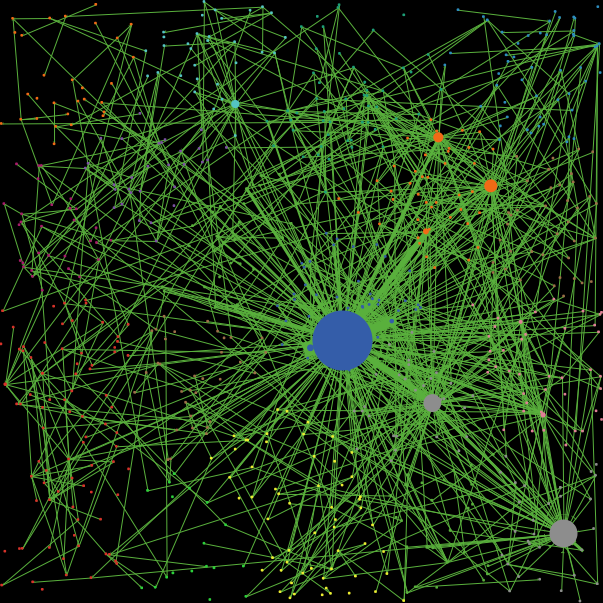
\includegraphics[width=0.48\textwidth]{figures/ex_alleq-highgravity_seed-12102_t1500.png}
    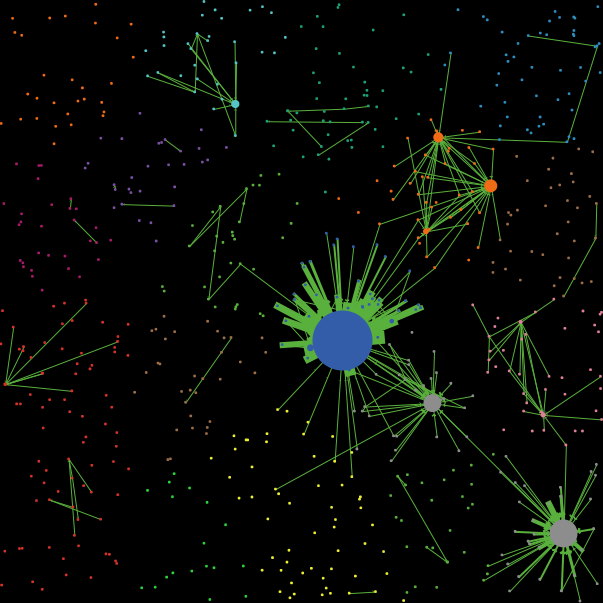
\includegraphics[width=0.48\textwidth]{figures/ex_alleq-lowgravity_seed-12102_t1500.png}\\
    \begin{mdframed}
    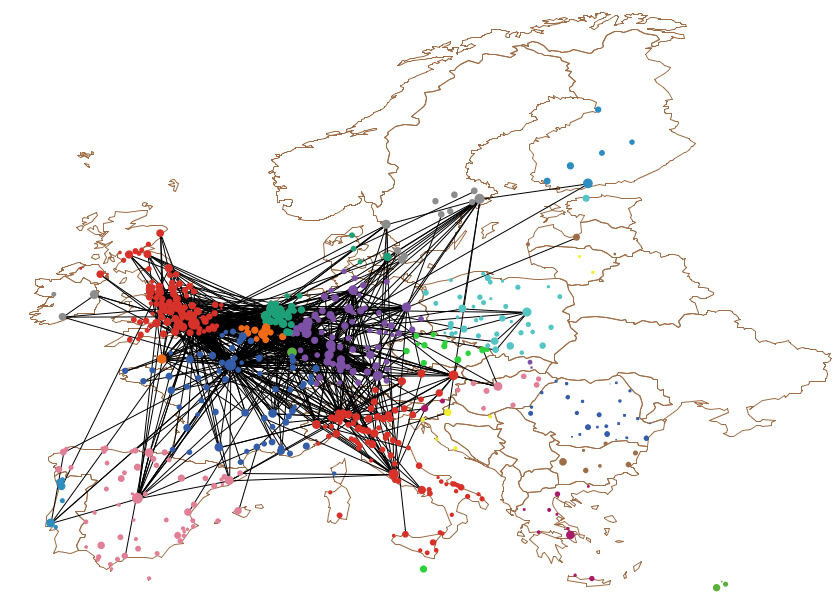
\includegraphics[width=0.48\textwidth]{figures/ex_real_highgravity_t1500.png}
    \end{mdframed}
    \begin{mdframed}
    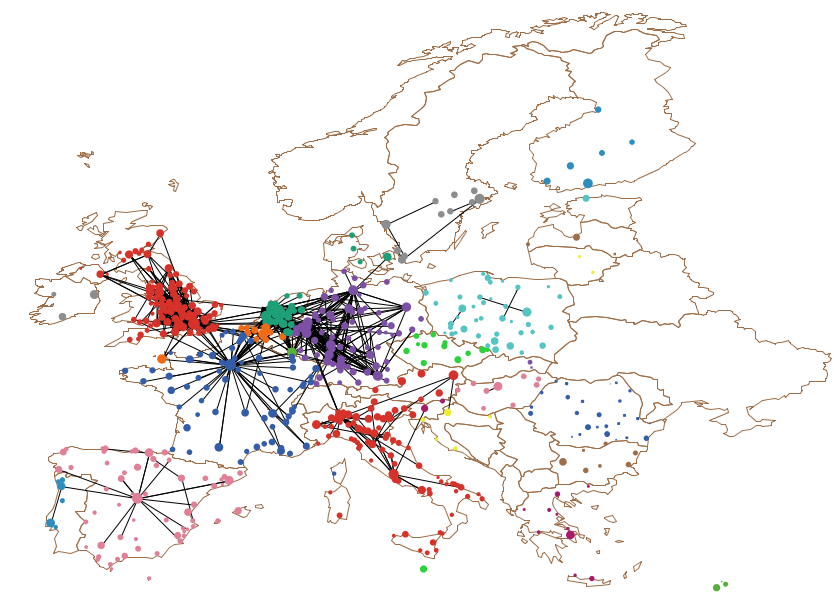
\includegraphics[width=0.48\textwidth]{figures/ex_real_lowgravity_t1500.png}
    \end{mdframed}
    \caption{Example of simulated networks at $t=1500$, for a synthetic system of cities (Top row) and the European urban network (Bottom row). , with a high (resp. low) gravity decay parameter for the left column (resp. right).\label{fig:example}}
\end{figure}
%%%%%%%%%%%%%


\subsection{Synthetic city systems}

\paragraph{Sensitivity analysis}


\paragraph{One factor sampling}
% 20190924_162740_ONEFACTOR_REPLICATIONS_SYNTHETIC_GRID

A first numerical experiment of one-factor sampling on all Cobb-Douglas parameters and 100 stochastic repetitions confirms a good statistical convergence (average Sharpe ratios for indicators all larger than 5). Behavior of some indicators are shown in Fig.~\ref{fig:onefactor}.

\begin{figure}
	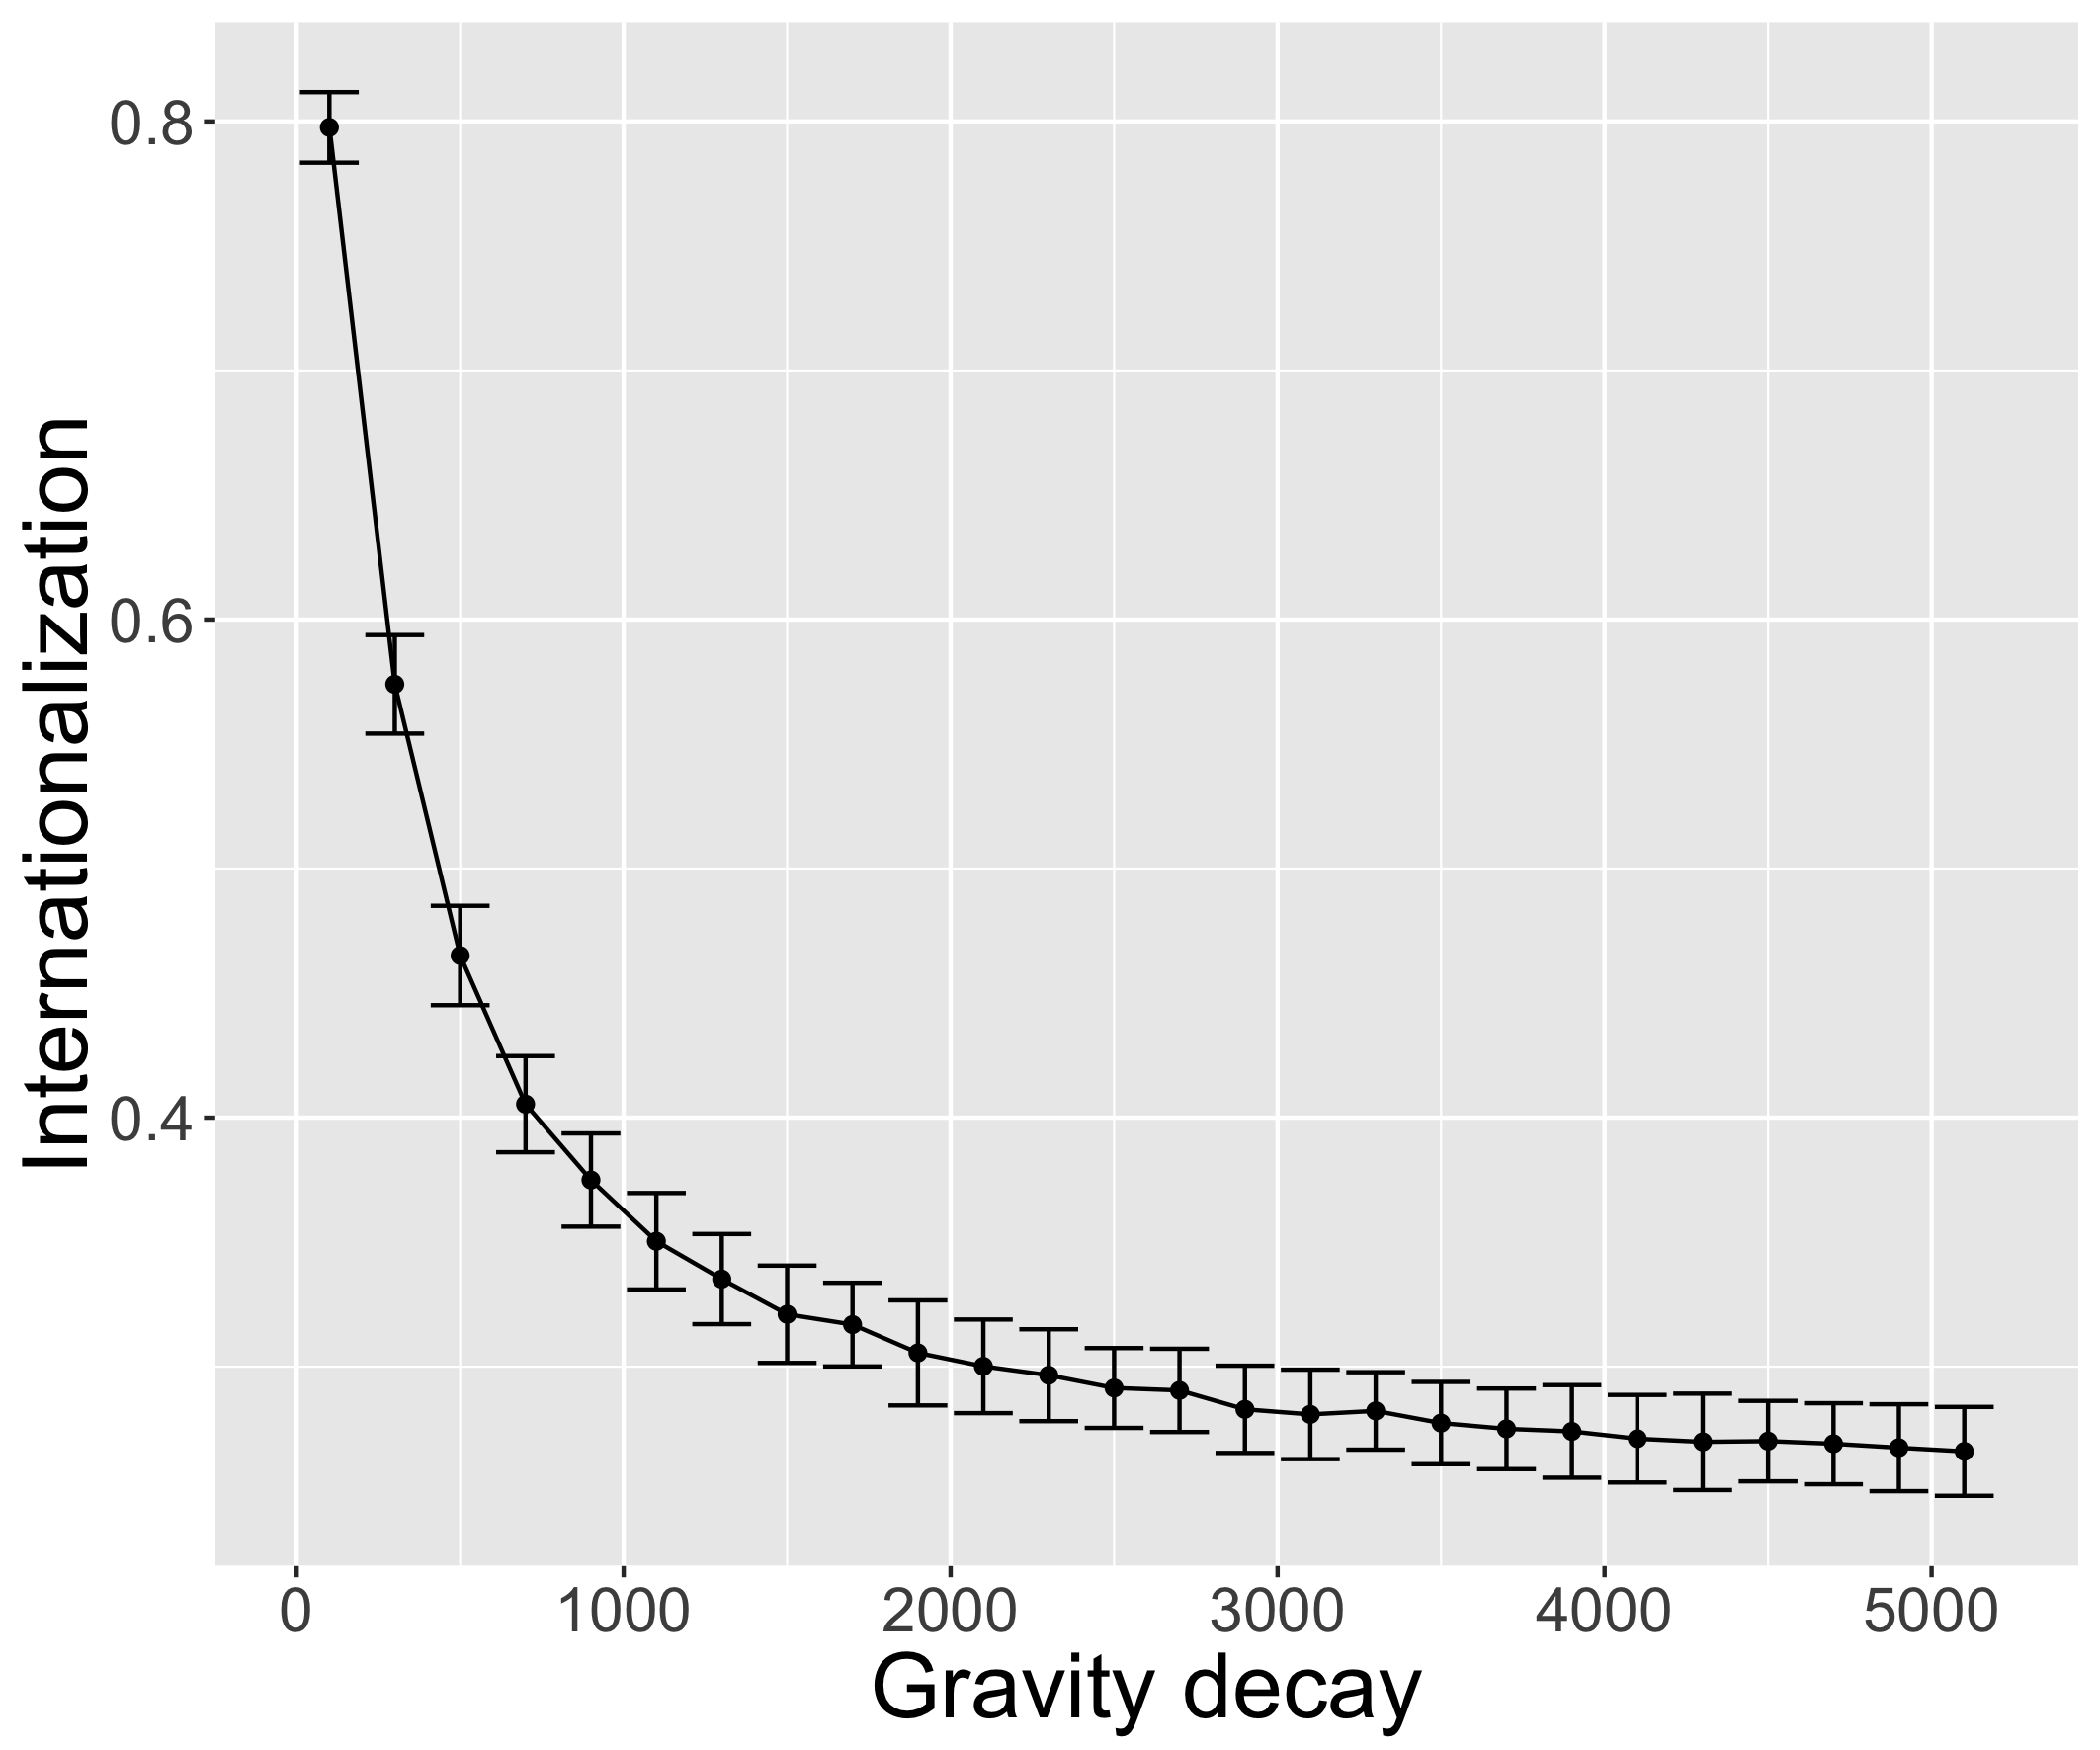
\includegraphics[width=0.48\textwidth,height=0.25\textheight]{figures/internationalization-gravityDecay_errorbars.png}
    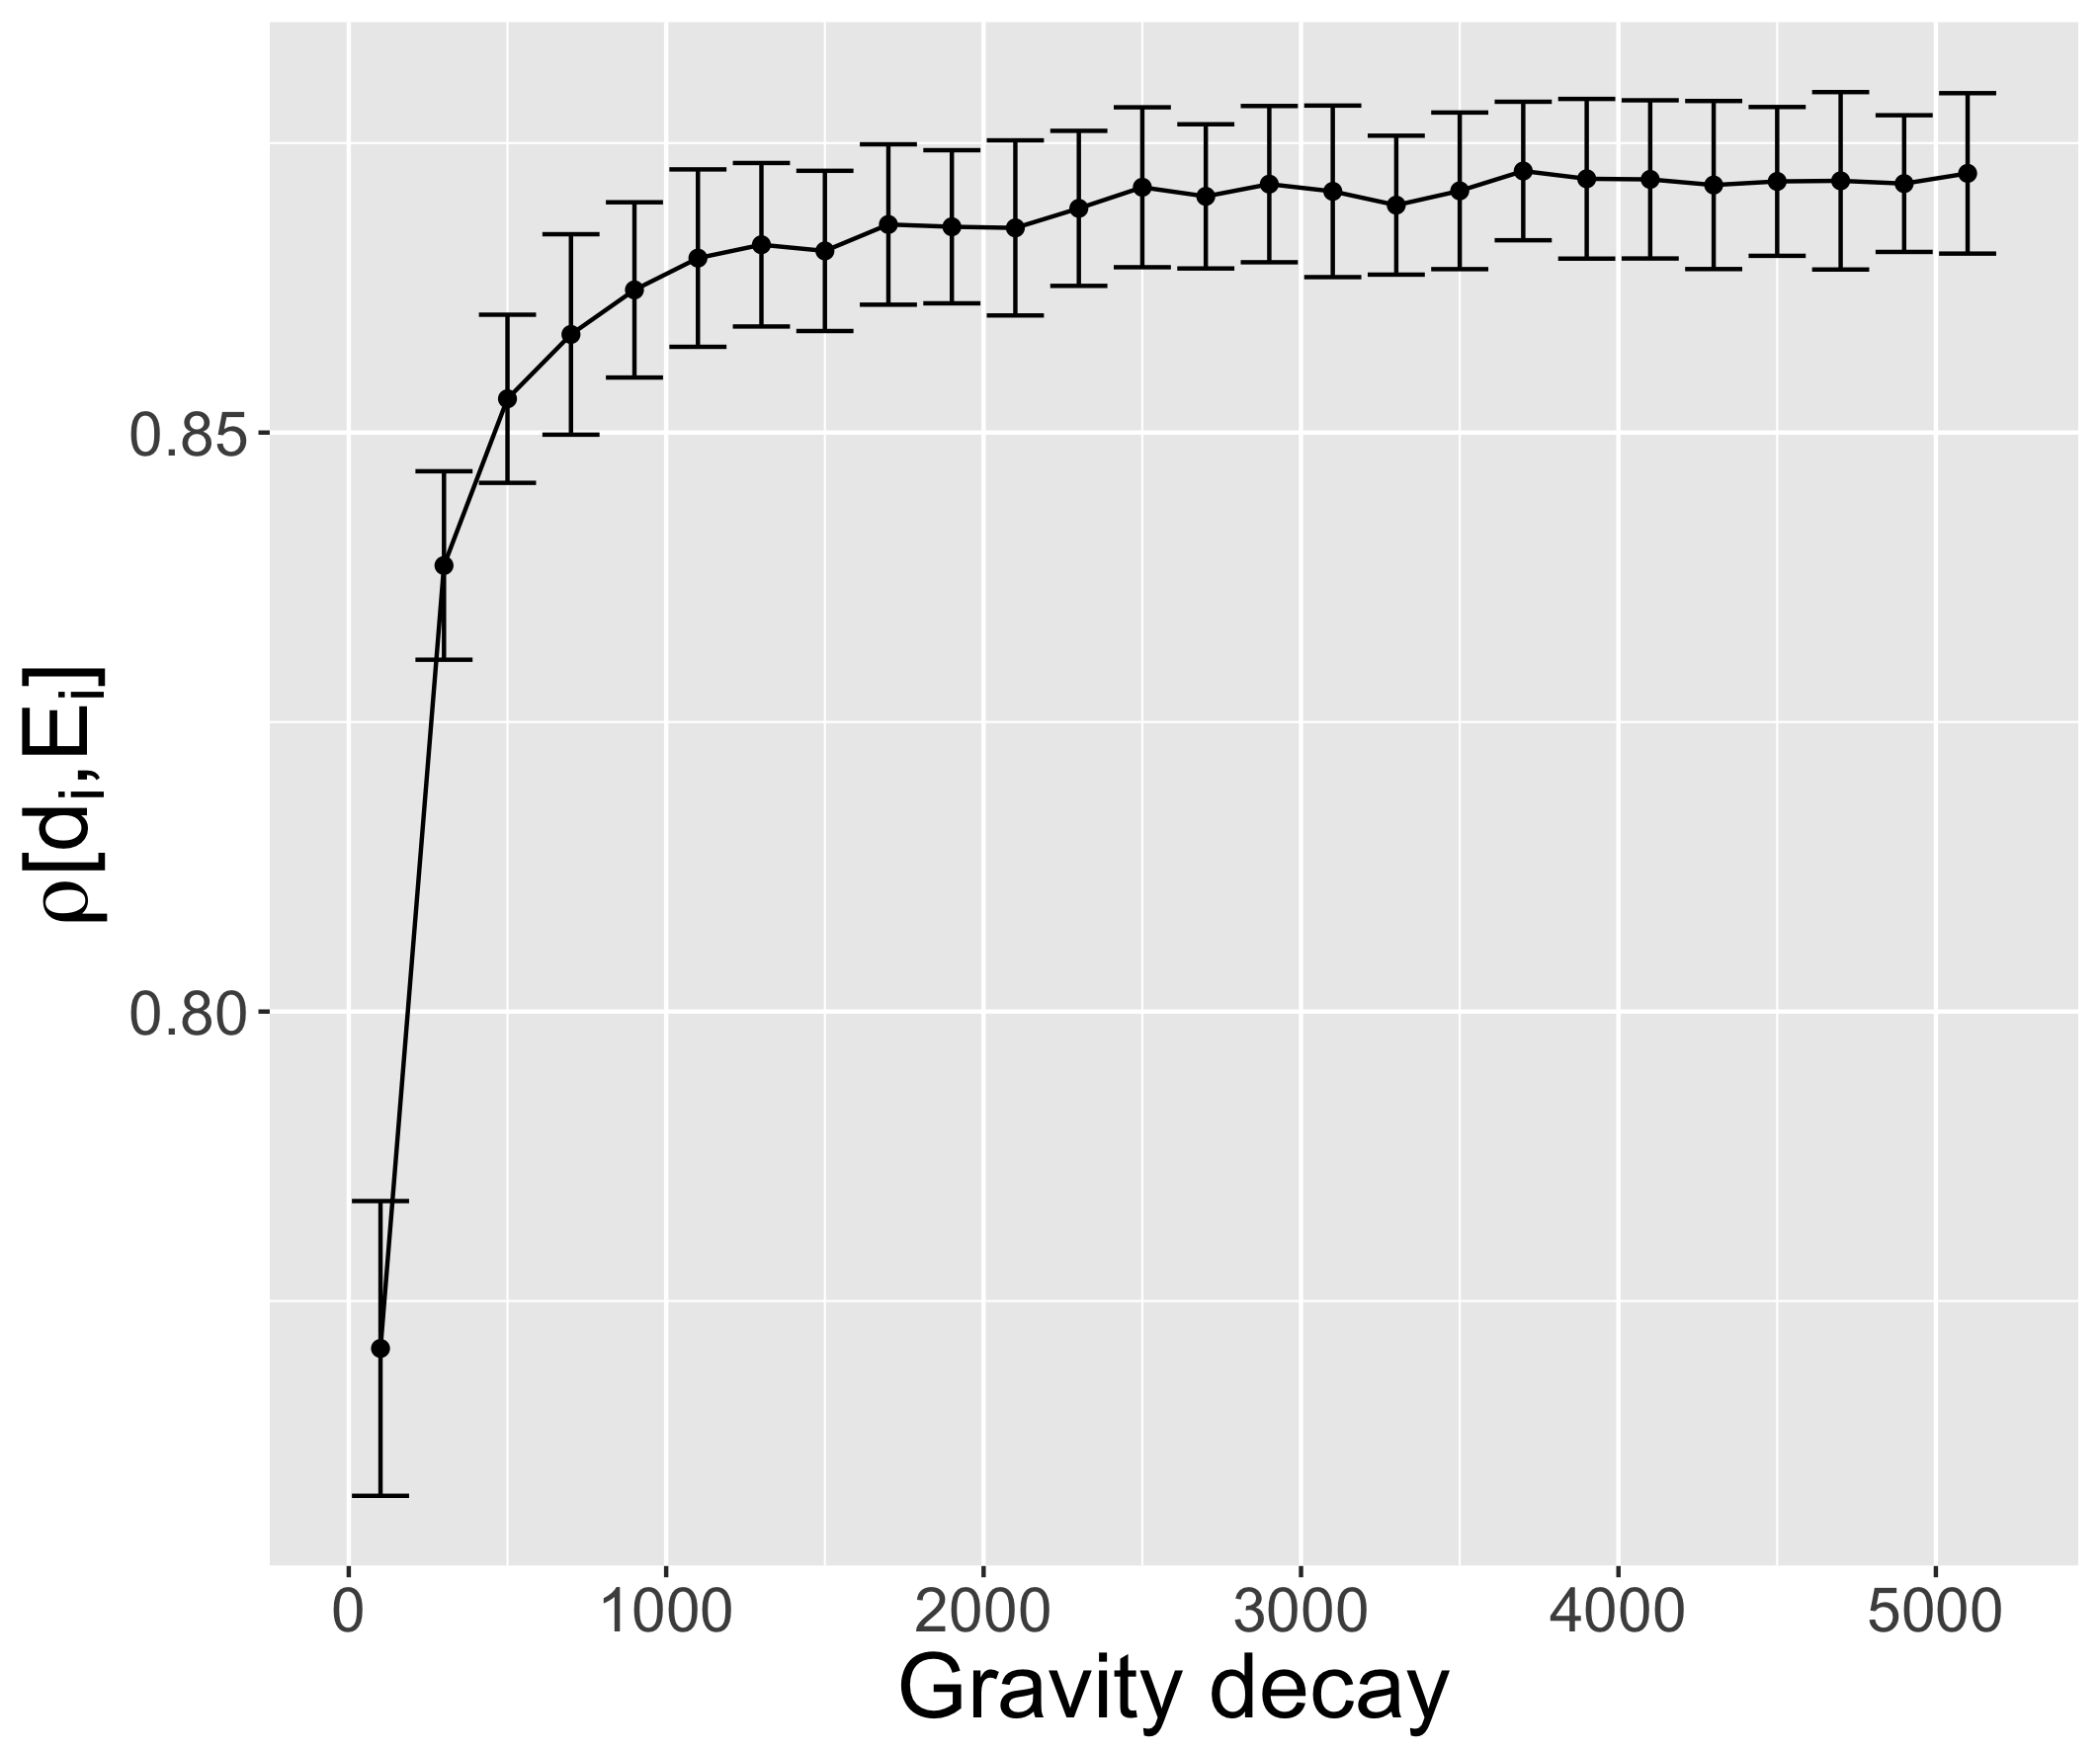
\includegraphics[width=0.48\textwidth,height=0.25\textheight]{figures/rhoDegreeSize-gravityDecay_errorbars.png}\\
    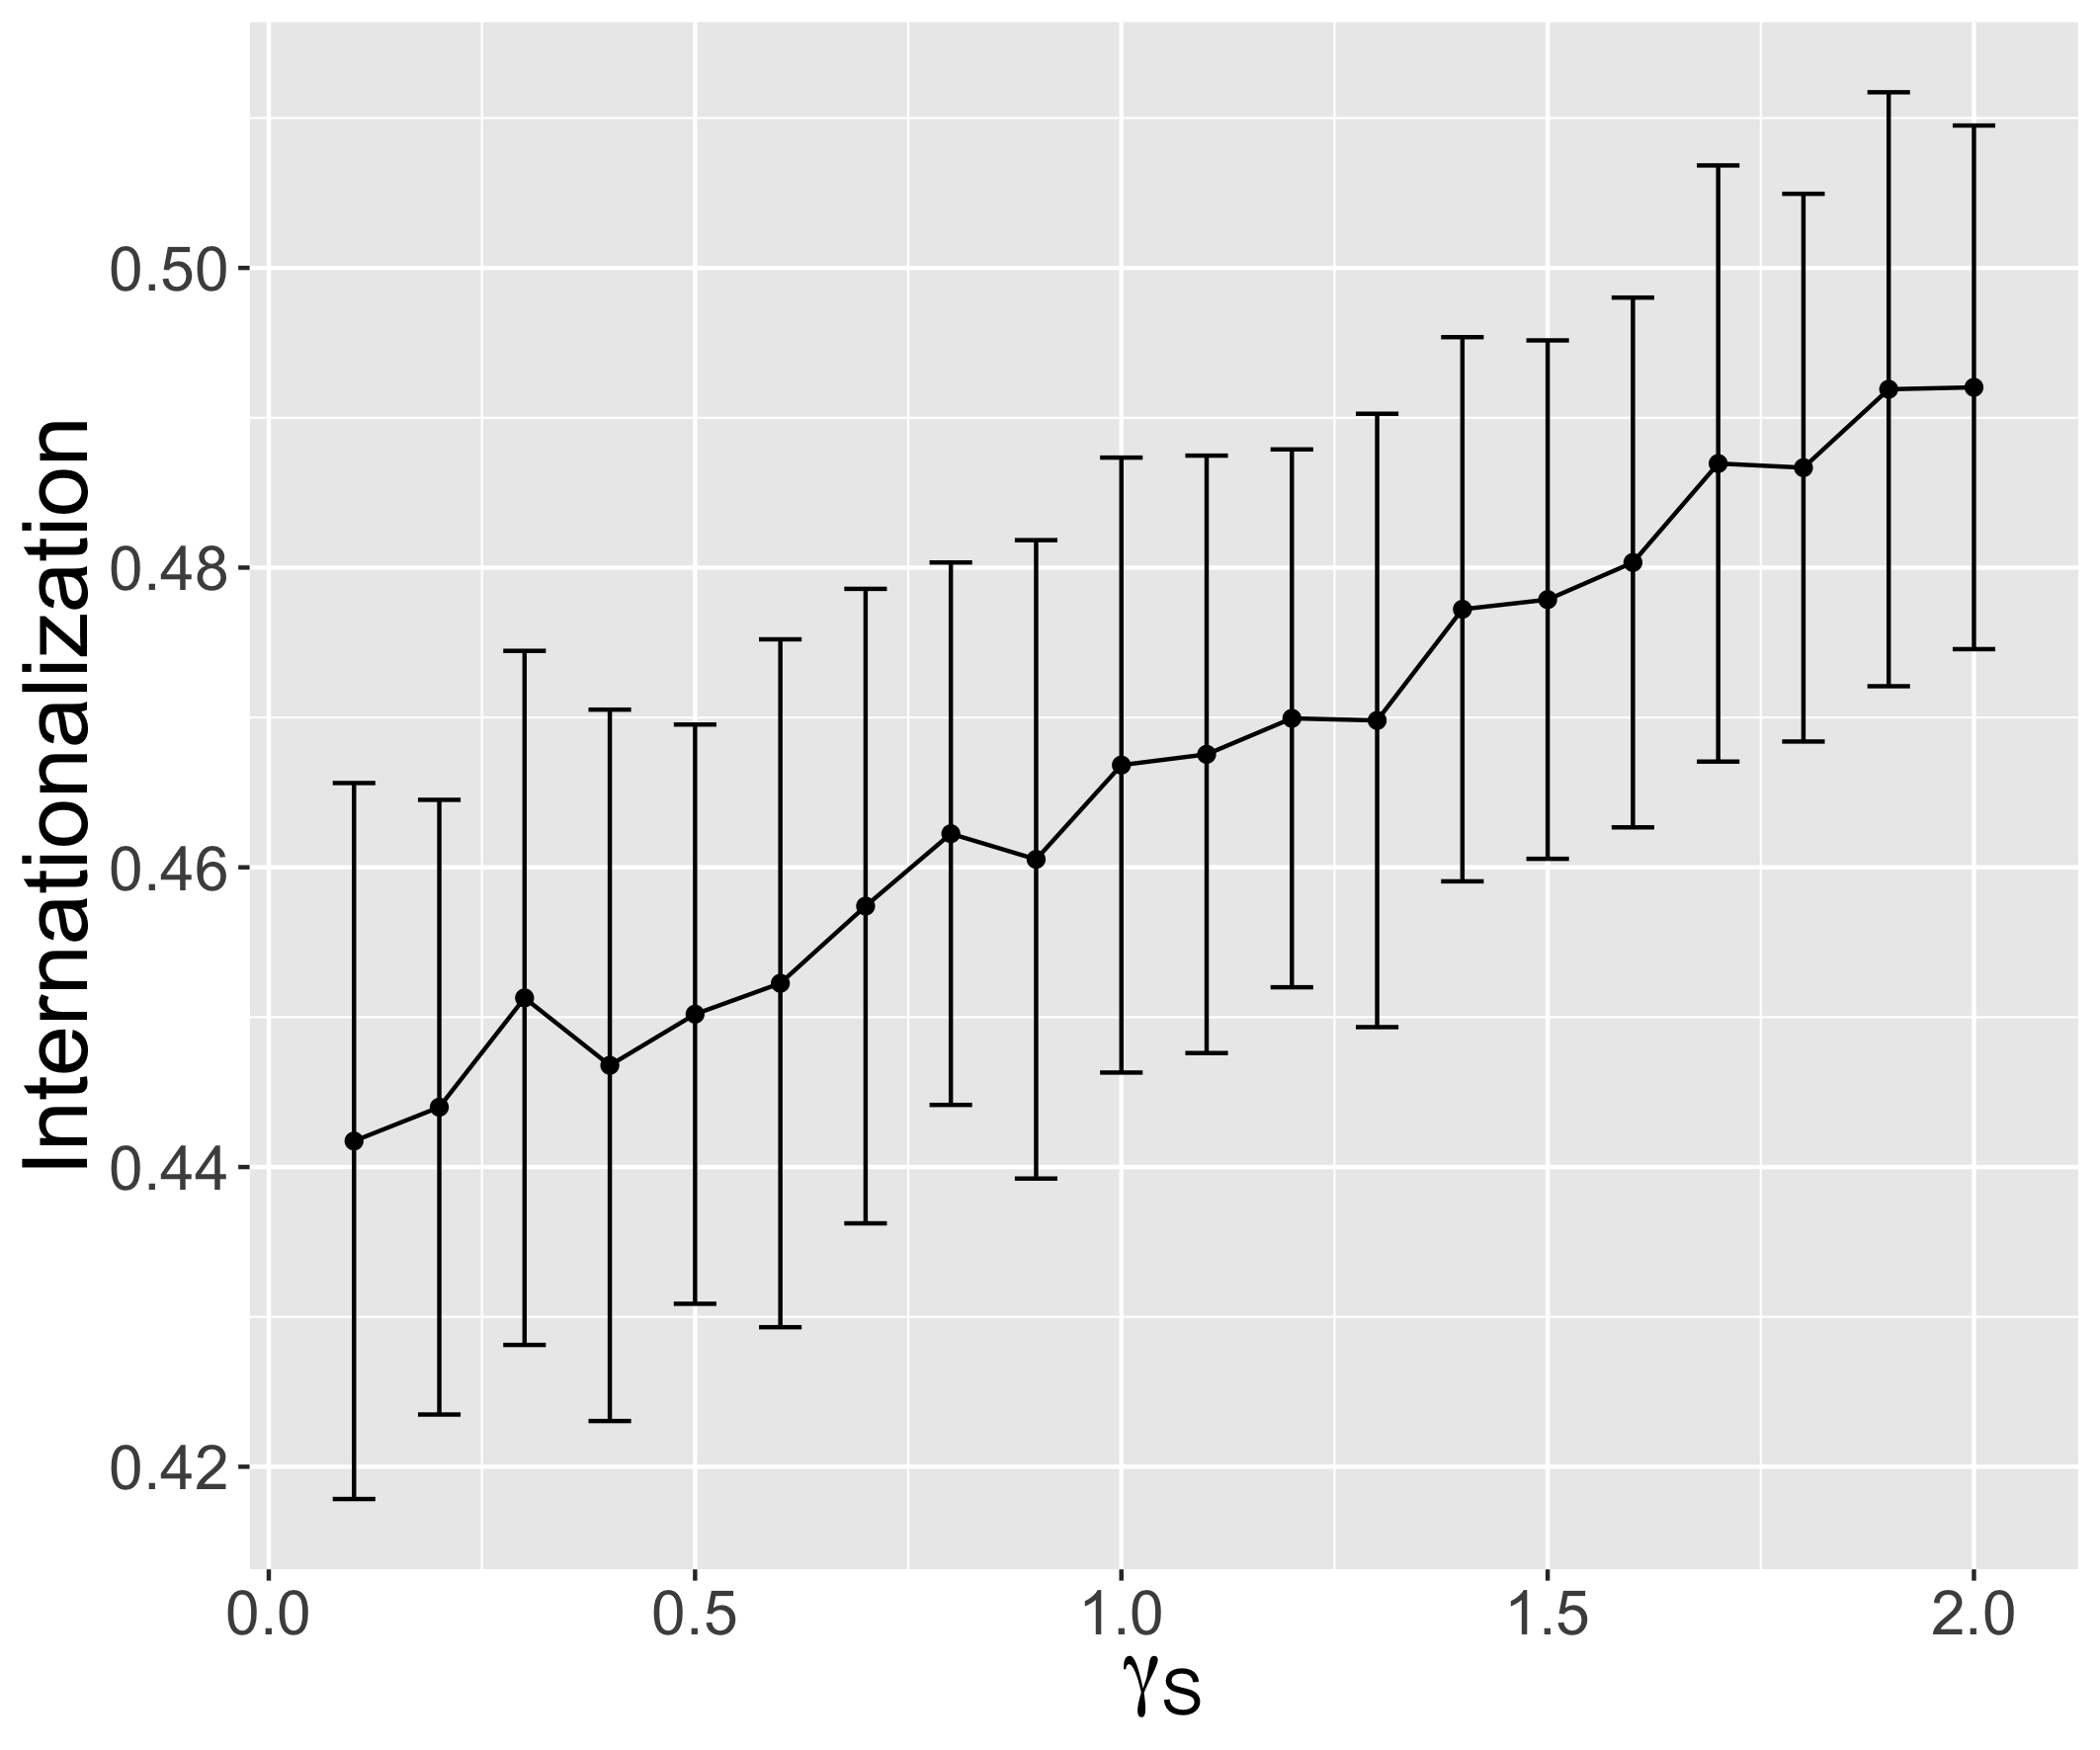
\includegraphics[width=0.48\textwidth,height=0.25\textheight]{figures/internationalization-gammaSectors_errorbars.png}
    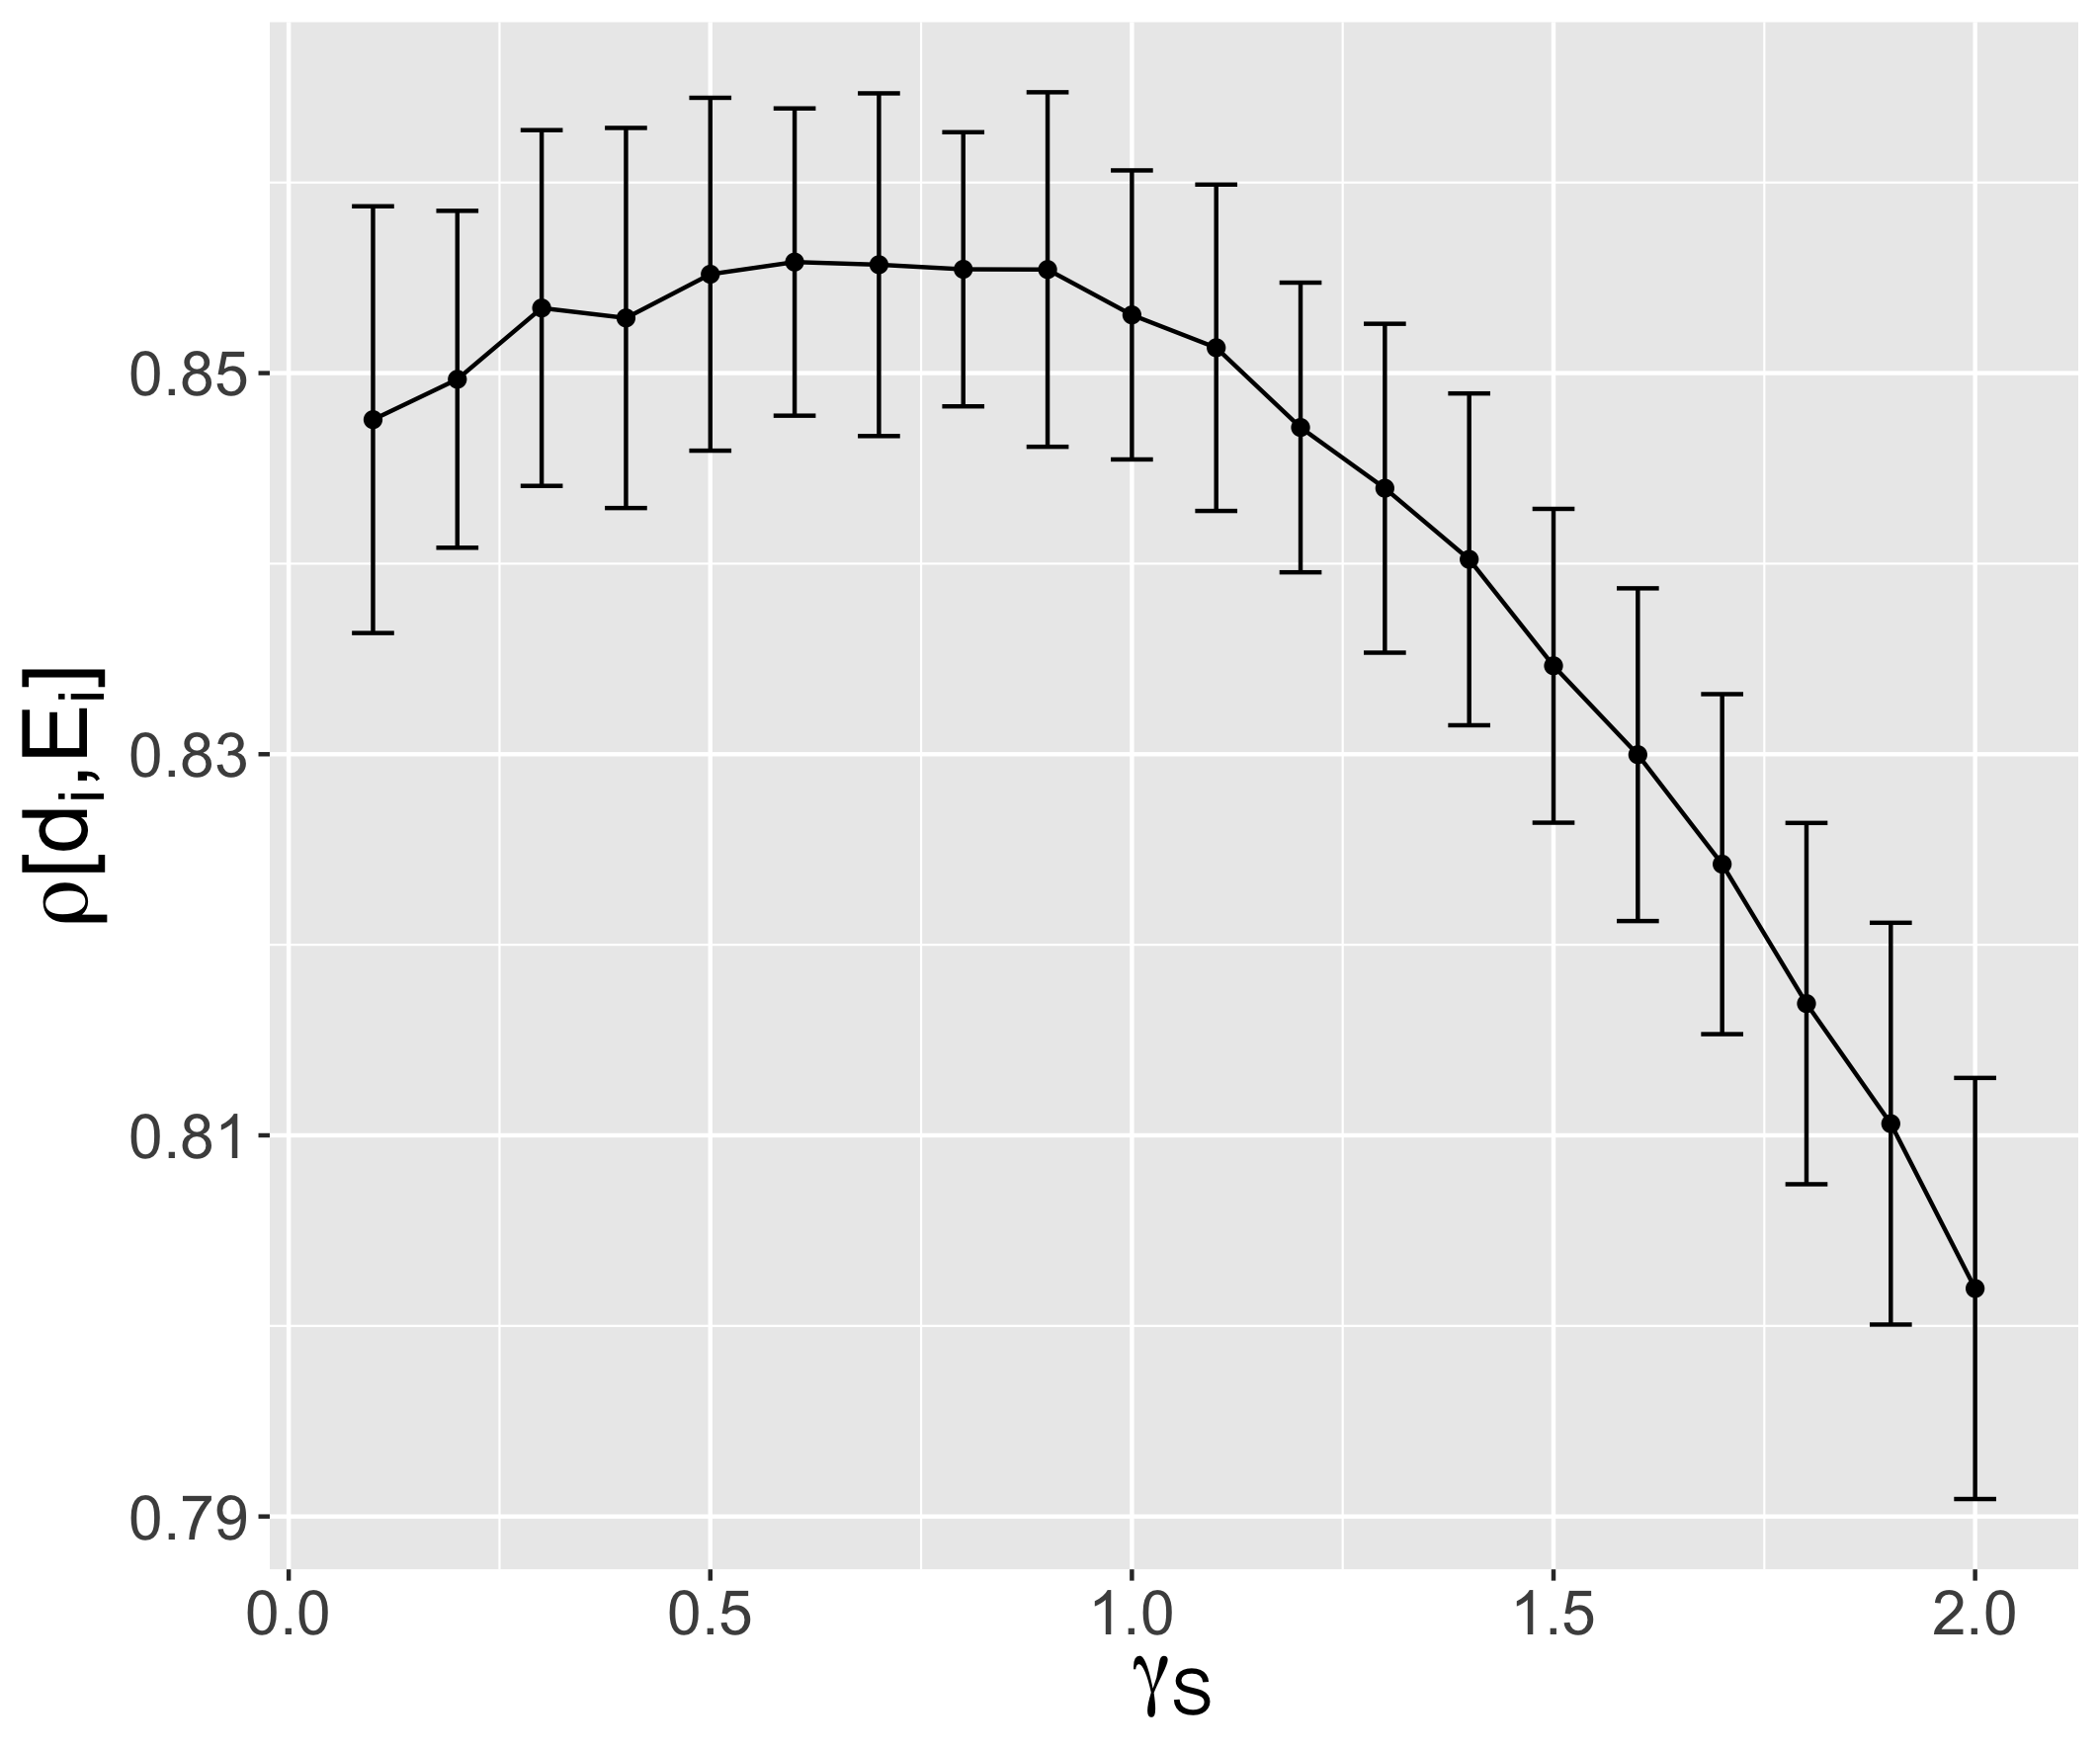
\includegraphics[width=0.48\textwidth,height=0.25\textheight]{figures/rhoDegreeSize-gammaSectors_errorbars.png}
    \caption{(Top Left) Internationalization index decreases exponentially with gravity decay; (Top Right) Correlation between city weighted degree and size. Both plots show a transition from a local to a global regime. (Bottom Left) Internationalization varies linearly with sector proximity $\gamma_S$; (Bottom Right) Correlation between degree and size exhibits a maximum, witnessing an intermediate regime where size is the most important. \label{fig:onefactor}}
\end{figure}



\paragraph{Grid exploration}

The model behaviour is then studied with a grid sampling for parameters and 20 repetitions (the computations run on the European Grid Infrastructure, and are equivalent to 2.5 years of CPU time).

The influence of gravity decay parameters is confirmed when plotting the internationalization index against the distance, which shows an exponential decay. Similarly, the correlation between city weighted degree and city size exhibit a behaviour that can be interpreted as a phase transition between local and global networks. Other indicators exhibit non-trivial patterns. For example, when considering average community size of the final network, we obtain a maximal integration in term of communities at an intermediate value of the gravity decay, what can be interpreted as the emergence of a regional regime. The size of communities is largely influenced by the value of the elasticities for the similarity function and the ratio of the economic output of the area. All these experiments reveal a complex interplay between processes and how the model produces diverse stylized facts.

\begin{figure}
    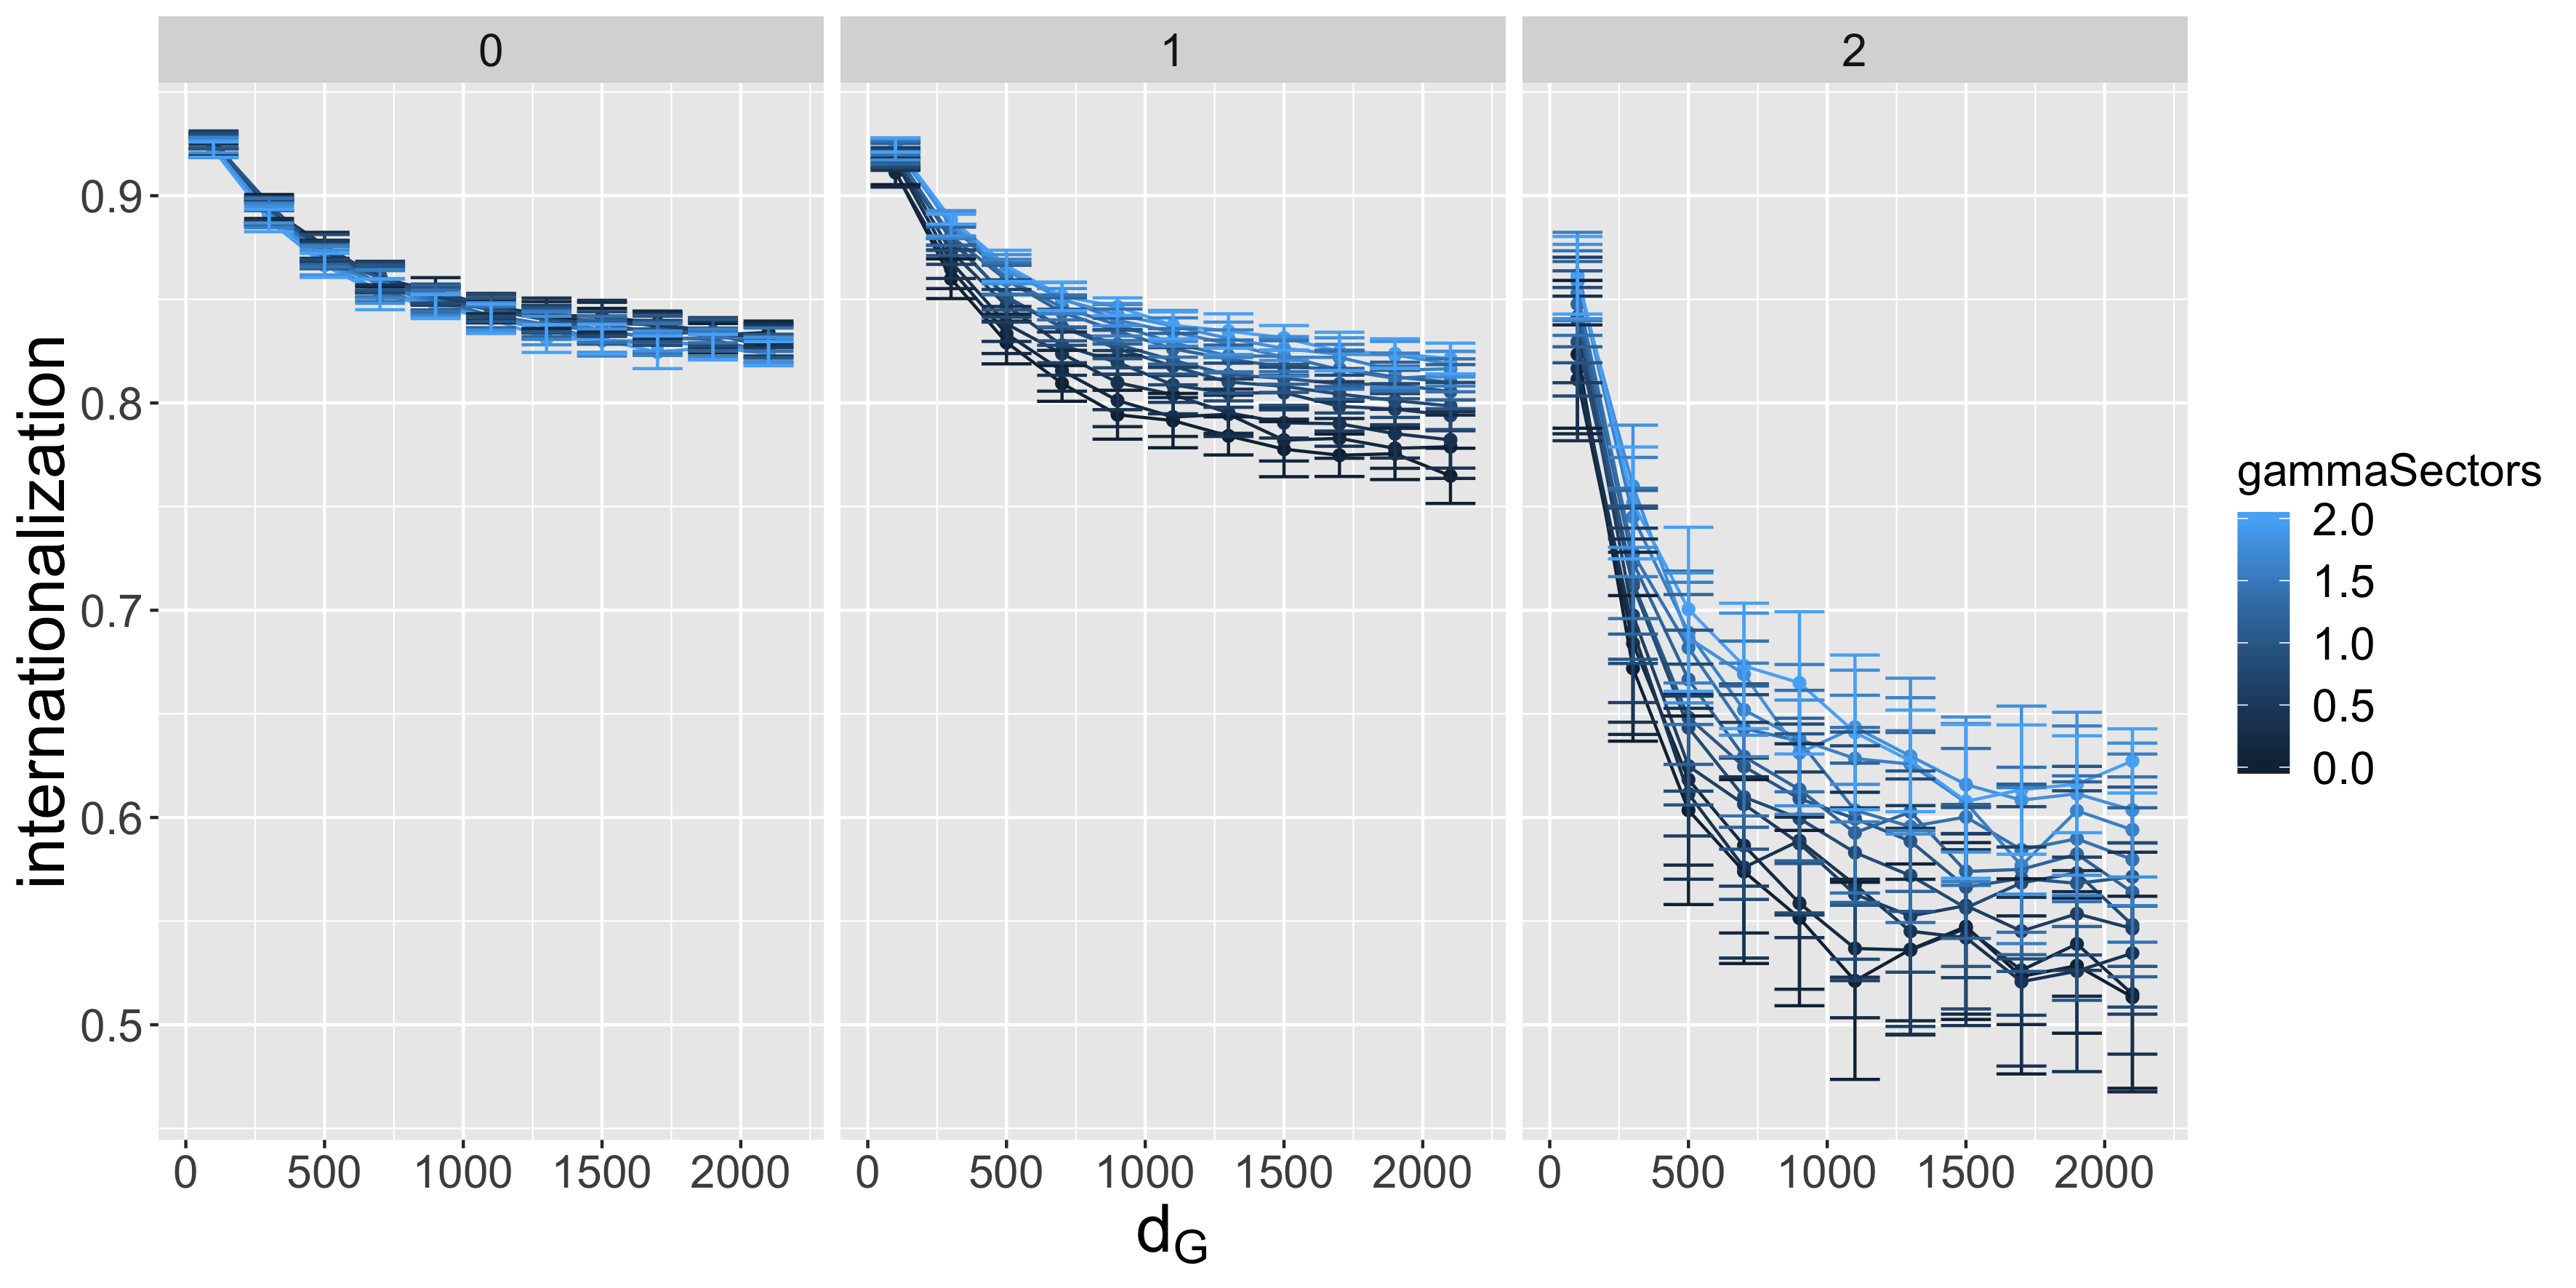
\includegraphics[width=\textwidth]{figures/internationalization_countryGravityDecay200_gammaDestination0_facetwrapgammaOrigin_colorgammaSectors.png}
    \caption{The transition as a function of interaction range depends on the influence of origin size $\gamma_F$; sector proximity $\gamma_S$ plays a role only for a large influence of the origin.}
\end{figure}



\begin{figure}
    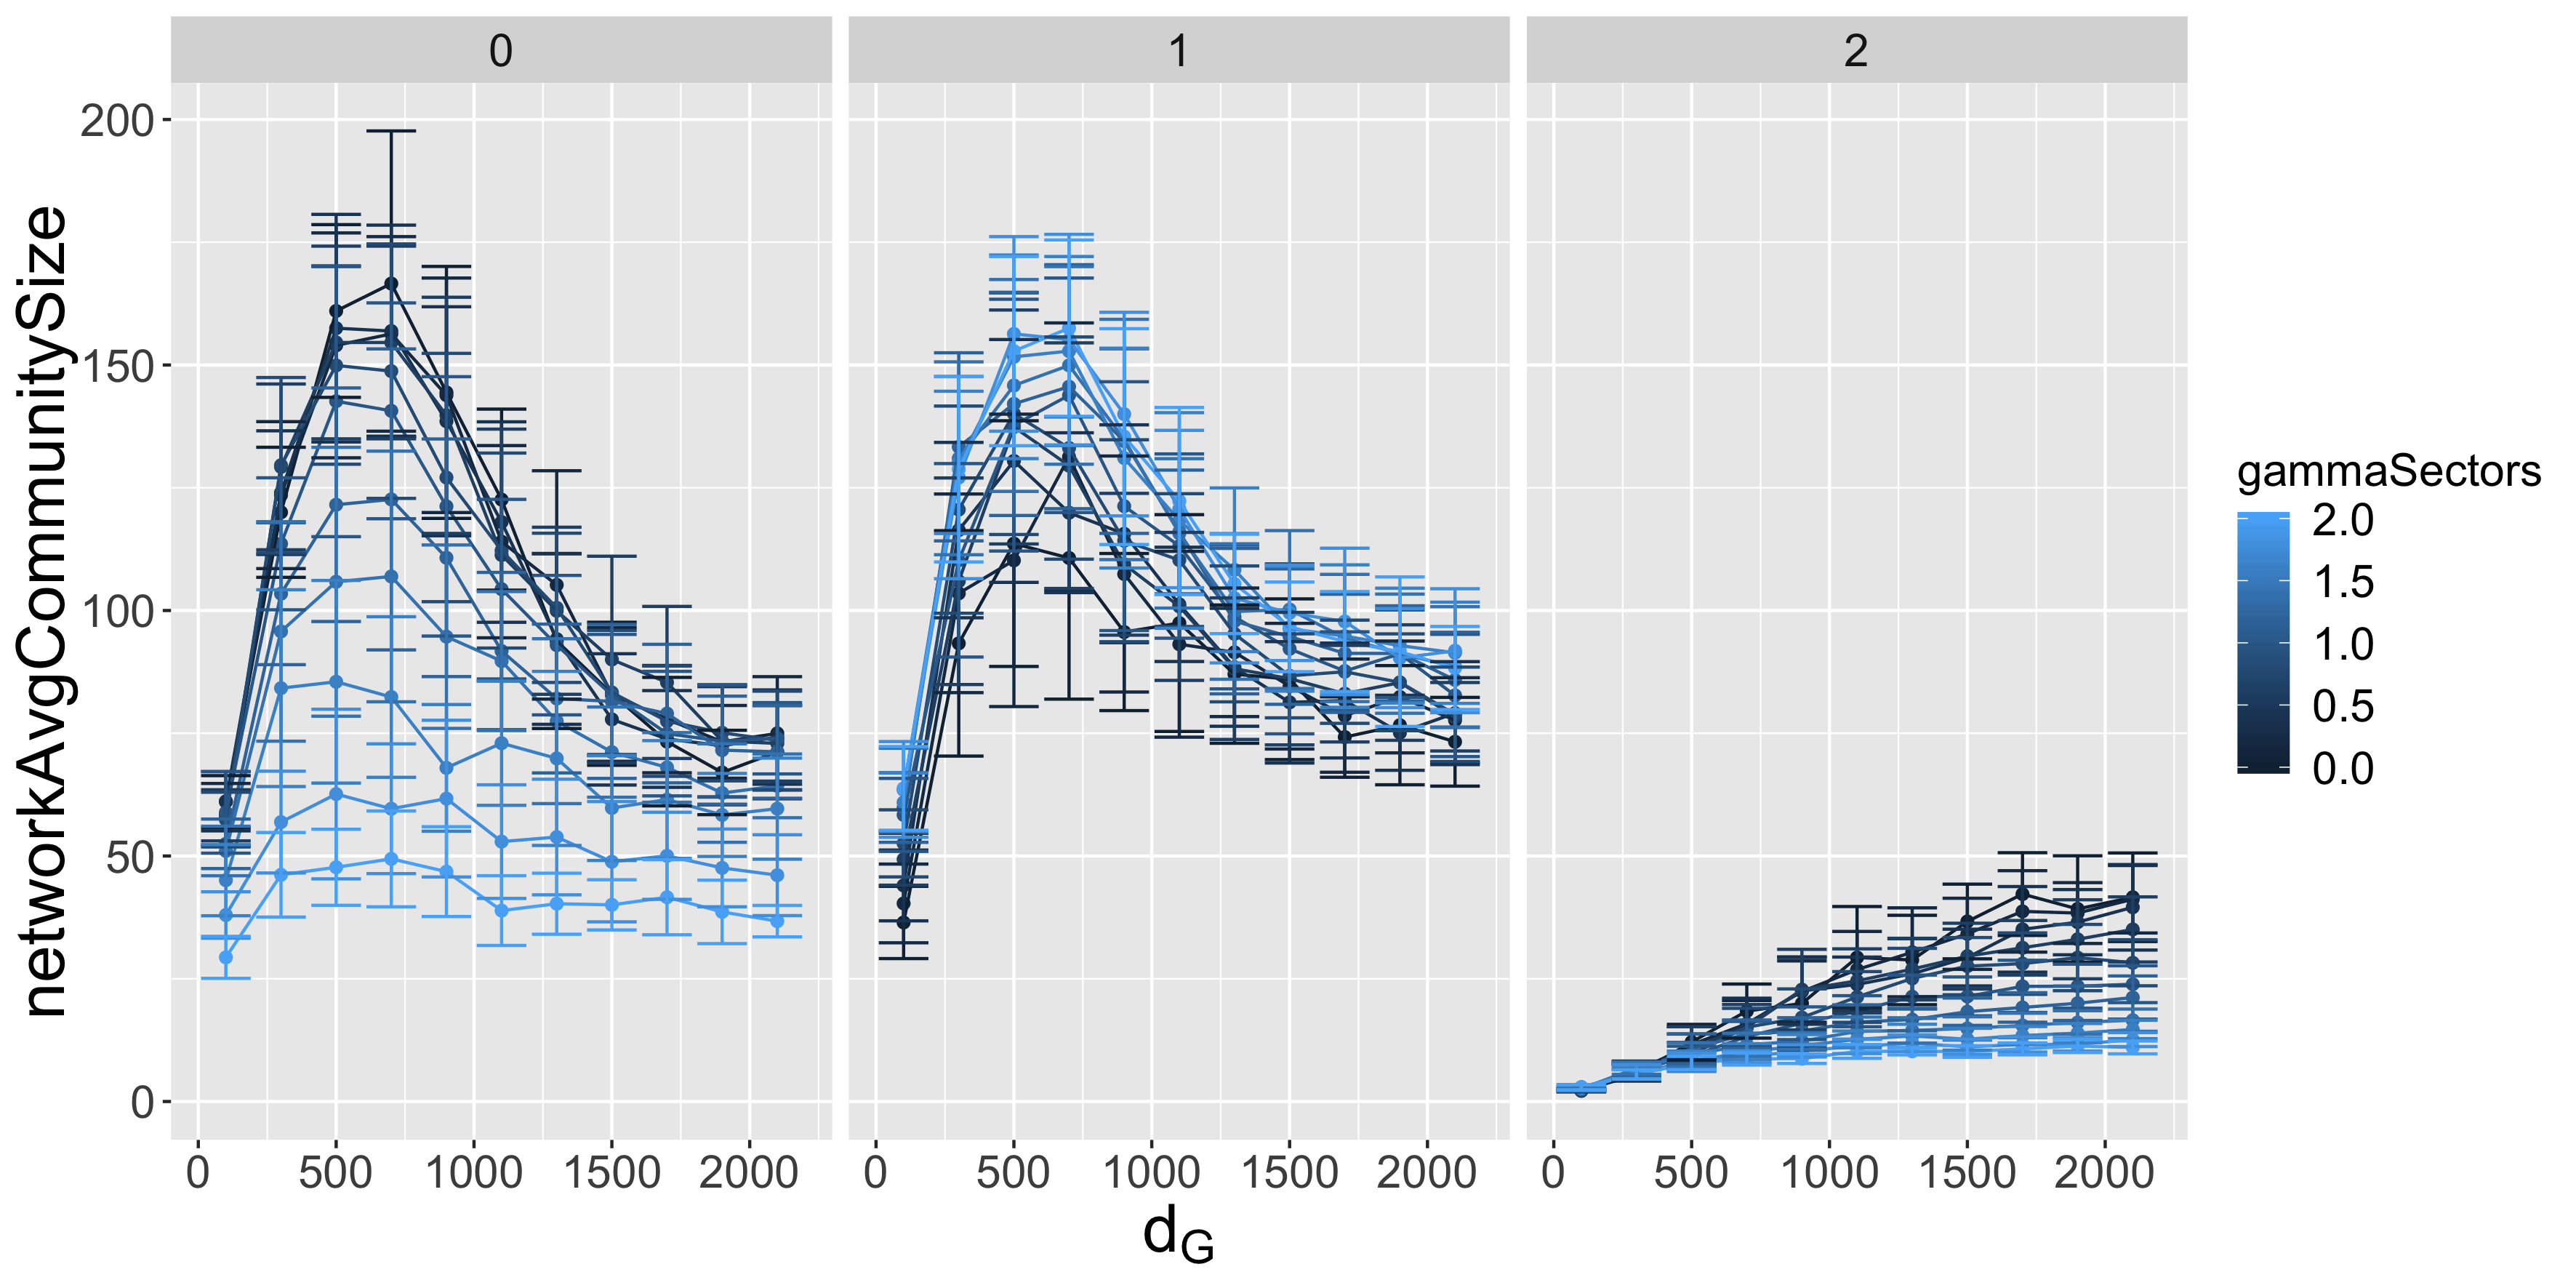
\includegraphics[width=\textwidth]{figures/networkAvgCommunitySize_countryGravityDecay2100_gammaDestination0_facetwrapgammaOrigin_colorgammaSectors.png}
	\caption{Maximal integration in term of community size is achieved at an intermediate value of $d_G$: emergence of a regional regime; Maximal size depends on the role of sectors $\gamma_S$, in a decreasing way when origin size is deactivated, and increasing way when $\gamma_F=1$; This regime disappear when origin size influence is too large}
\end{figure}




% Saltelli exploration of the model
% -> confirm relative importance of params and search for inhomogeneity/interaction effects


\subsection{Model calibration on the European urban network}


As a matter of validation, the model is implemented for real data for Europe joining Functional Urban Areas with the Global Human Settlement Database for cities and their characteristics, with the AMADEUS database produced by the Bureau Van Dijk on ownership links between firms in Europe in 2018 at postcode level in all types of sectors.



\subsubsection{Model calibration}

Calibration is done using a genetic NSGA2 algorithm, finding the parameter values giving network trajectories closest to reality. First results show in particular a role of the path-dependency parameter confirming the relevance of this complex generative model. Further work is needed to get more interpretations from this experiment, but our study demonstrates the feasibility of model calibration on real data. Several scenarios are considered taking into consideration the current and future economic challenges, such as those given by Brexit. The model may be applied in future work to assess policy issues and recommendations.




%%%%%%%%%%%%%%%
\section{Discussion}

This paper aimed at presenting a generative model for urban networks defined by interactions between firms based on synthetic data, simulated thanks to OpenMole and calibrated on real data on ownership linkages of firms for Europe. The simulation on a synthetic system of cities unveil phase transitions when changing interaction distance, and non-trivial patterns in the model behavior. This kind of model can have practical application in the future in terms of testing the effect of exogenous shocks in the socio-economic structure as the upcoming effect of Brexit on the European market.

Even in such a simple model (close to directly tractable stationary state) the behaviour is highly non-linear in many dimensions. Our study shows how crucial model exploration is to overcome hidden parameters (deactivated mechanisms or default parameter values). This paper emphasis on the fact that exploration of intrinsic dynamics on synthetic data is of great importance should be driven before an application on real data so as to put aside the geographical effects from model dynamics.

Several possible extensions of the current work can be undertaken in the future as a co-evolution model with an evolution of city sizes or a model with firm agents leading to a multi-scale agent-based model. A more precise study of the role of path dependency can also be undertaken in the creation of the links. Other formulations of the model might be taken into consideration as other formulation of the combination of factors or multi-objective optimisation depending on sectors using Pareto fronts.  

% - other formulation of the combination of factors
%multi-objective optimization depending on sectors, using Pareto fronts ? - needs empirical evidence; (iv) copula-based combination as done by \cite{2019arXiv190505106C} - copula parameters are free or estimated from real data
% The function used can be understood as a separable spatial interaction model. As a possible extension, Copula capture a dependency structure but must be parametrised by estimation on real data.

% - evolution of city sizes (co-evolution model)
% - role of path dependency
% - towards a model with firm agents? (multi-scale ABM)


\bibliographystyle{apalike}
%\bibliographystyle{unsrt}
\bibliography{biblio}

\end{document}
